%&preformat-synopsis
\RequirePackage[l2tabu,orthodox]{nag} % Раскомментировав, можно в логе получать рекомендации относительно правильного использования пакетов и предупреждения об устаревших и нерекомендуемых пакетах

% Откомментируйте, чтобы отключить генерацию закладок в pdf
% \PassOptionsToPackage{bookmarks=false}{hyperref}
\documentclass[a5paper,10pt,twoside,openany,article]{memoir} %,draft

\AtBeginDocument{\linespread{0.98}\selectfont} % поджатие текста, так чтобы освободить 28 страницу

% --- Компактные заголовки: без отбивок сверху/снизу ---
\setbeforesecskip{0pt plus 0pt minus 0pt}
\setaftersecskip{0.1pt plus 0pt minus 0pt}
\setbeforesubsecskip{0pt plus 0pt minus 0pt}
\setaftersubsecskip{0pt plus 0pt minus 0pt}
\setbeforesubsubsecskip{0pt plus 0pt minus 0pt}
\setaftersubsubsecskip{0pt plus 0pt minus 0pt}

% --- Убираем «резиновые» и абзацные отступы ---
\setlength{\parskip}{0pt}
\setlength{\parindent}{1.25em}   % при желании можно оставить
\setlength{\topsep}{0pt}
\setlength{\partopsep}{0pt}
\setlength{\parsep}{0pt}
\setlength{\itemsep}{0pt}

% --- Страницы тянем не по нижнему краю, а по содержимому ---
\raggedbottom

\input{common/setup}          % общие настройки шаблона
%%% Проверка используемого TeX-движка %%%
\newif\ifxetexorluatex   % определяем новый условный оператор (http://tex.stackexchange.com/a/47579)
\ifxetex
    \xetexorluatextrue
\else
    \ifluatex
        \xetexorluatextrue
    \else
        \xetexorluatexfalse
    \fi
\fi

\newif\ifsynopsis           % Условие, проверяющее, что документ --- автореферат

\usepackage{etoolbox}[2015/08/02]   % Для продвинутой проверки разных условий
\providebool{presentation}

\usepackage{comment}    % Позволяет убирать блоки текста (добавляет
                        % окружение comment и команду \excludecomment)

%%% Поля и разметка страницы %%%
\usepackage{pdflscape}  % Для включения альбомных страниц
\usepackage{geometry}   % Для последующего задания полей

%%% Таблица на 90 градусов %%%
\usepackage{rotating}

%%% Настройки для алгоритмов %%%
\usepackage{algorithm}
\floatname{algorithm}{Алгоритм}
\usepackage{algpseudocode}

\makeatletter
\newenvironment{breakablealgorithm}
{% \begin{breakablealgorithm}
		\begin{center}
			\refstepcounter{algorithm}% New algorithm
			\hrule height.8pt depth0pt \kern2pt% \@fs@pre for \@fs@ruled
			\renewcommand{\caption}[2][\relax]{% Make a new \caption
				{\raggedright\textbf{\fname@algorithm~\thealgorithm} ##2\par}%
				\ifx\relax##1\relax % #1 is \relax
				\addcontentsline{loa}{algorithm}{\protect\numberline{\thealgorithm}##2}%
				\else % #1 is not \relax
				\addcontentsline{loa}{algorithm}{\protect\numberline{\thealgorithm}##1}%
				\fi
				\kern2pt\hrule\kern2pt
			}
		}{% \end{breakablealgorithm}
		\kern2pt\hrule\relax% \@fs@post for \@fs@ruled
	\end{center}
}
\makeatother

%%% Математические пакеты %%%
\usepackage{amsthm,amsmath,amscd}   % Математические дополнения от AMS
\usepackage{amsfonts,amssymb}       % Математические дополнения от AMS
\usepackage{mathtools}              % Добавляет окружение multlined
\usepackage{xfrac}                  % Красивые дроби
\usepackage[
    locale = DE,
    list-separator       = {;\,},
    list-final-separator = {;\,},
    list-pair-separator  = {;\,},
    list-units           = single,
    range-units          = single,
    range-phrase={\text{\ensuremath{-}}},
    % quotient-mode        = fraction, % красивые дроби могут не соответствовать ГОСТ
    fraction-function    = \sfrac,
    separate-uncertainty,
    ]{siunitx}[=v2]                 % Размерности SI
\sisetup{inter-unit-product = \ensuremath{{}\cdot{}}}

\DeclareMathOperator*{\argmax}{arg\,max}
\DeclareMathOperator*{\argmin}{arg\,min}

% Кириллица в нумерации subequations
% Для правильной работы требуется выполнение сразу после загрузки пакетов
\patchcmd{\subequations}{\def\theequation{\theparentequation\alph{equation}}}
{\def\theequation{\theparentequation\asbuk{equation}}}
{\typeout{subequations patched}}{\typeout{subequations not patched}}

%%%% Установки для размера шрифта 14 pt %%%%
%% Формирование переменных и констант для сравнения (один раз для всех подключаемых файлов)%%
%% должно располагаться до вызова пакета fontspec или polyglossia, потому что они сбивают его работу
\newlength{\curtextsize}
\newlength{\bigtextsize}
\setlength{\bigtextsize}{13.9pt}

\makeatletter
%\show\f@size    % неплохо для отслеживания, но вызывает стопорение процесса,
                 % если документ компилируется без команды  -interaction=nonstopmode
\setlength{\curtextsize}{\f@size pt}
\makeatother

%%% Кодировки и шрифты %%%
\ifxetexorluatex
    \ifpresentation
        \providecommand*\autodot{} % quick fix for polyglossia 1.50
    \fi
    \PassOptionsToPackage{no-math}{fontspec}    % https://tex.stackexchange.com/a/26295/104425
    \usepackage{polyglossia}[2014/05/21]        % Поддержка многоязычности
                                        % (fontspec подгружается автоматически)
\else
   %%% Решение проблемы копирования текста в буфер кракозябрами
    \ifnumequal{\value{usealtfont}}{0}{}{
        \input glyphtounicode.tex
        \input glyphtounicode-cmr.tex %from pdfx package
        \pdfgentounicode=1
    }
    \usepackage{cmap}   % Улучшенный поиск русских слов в полученном pdf-файле
    \ifnumequal{\value{usealtfont}}{2}{}{
        \defaulthyphenchar=127  % Если стоит до fontenc, то переносы
                                % не впишутся в выделяемый текст при
                                % копировании его в буфер обмена
    }
    \usepackage{textcomp}
    \usepackage[T1,T2A]{fontenc}                    % Поддержка русских букв
    \ifnumequal{\value{usealtfont}}{1}{% Используется pscyr, при наличии
        \IfFileExists{pscyr.sty}{\usepackage{pscyr}}{}  % Подключение pscyr
    }{}
    \usepackage[utf8]{inputenc}[2014/04/30]         % Кодировка utf8
    \usepackage[english, russian]{babel}[2014/03/24]% Языки: русский, английский
    \makeatletter\AtBeginDocument{\let\@elt\relax}\makeatother % babel 3.40 fix
    \ifnumequal{\value{usealtfont}}{2}{
        % http://dxdy.ru/post1238763.html#p1238763
        \usepackage[scaled=0.914]{XCharter}[2017/12/19] % Подключение русифицированных шрифтов XCharter
        \usepackage[charter, vvarbb, scaled=1.048]{newtxmath}[2017/12/14]
        \ifpresentation
        \else
            \setDisplayskipStretch{-0.078}
        \fi
    }{}
\fi

%%% Оформление абзацев %%%
\ifpresentation
\else
    \indentafterchapter     % Красная строка после заголовков типа chapter
    \usepackage{indentfirst}
\fi

%%% Цвета %%%
\ifpresentation
\else
    \usepackage[dvipsnames, table, hyperref]{xcolor} % Совместимо с tikz
\fi

%%% Таблицы %%%
\usepackage{longtable} % Длинные таблицы
\usepackage{multirow,makecell}   % Улучшенное форматирование таблиц
\usepackage{tabulary,tabularray} % Таблицы с автоматически подбирающейся
                                 % шириной столбцов
\UseTblrLibrary{booktabs}
\ExplSyntaxOn% define \IfTokenListEmpty to use \captionof with tabularray
\prg_generate_conditional_variant:Nnn \tl_if_empty:n { e } { TF }
\let \IfTokenListEmpty = \tl_if_empty:eTF
\ExplSyntaxOff

\usepackage{threeparttable}      % автоматический подгон ширины подписи таблицы

%%% Общее форматирование
%\usepackage{soul}% Поддержка переносоустойчивых подчёркиваний и зачёркиваний
\usepackage{icomma}  % Запятая в десятичных дробях

%%% Оптимизация расстановки переносов и длины последней строки абзаца
\IfFileExists{impnattypo.sty}{% проверка установленности пакета impnattypo
    \ifluatex
        \ifnumequal{\value{draft}}{1}{% Черновик
            \usepackage[hyphenation, lastparline, nosingleletter, homeoarchy,
            rivers, draft]{impnattypo}
        }{% Чистовик
            \usepackage[hyphenation, lastparline, nosingleletter]{impnattypo}
        }
    \else
        \usepackage[hyphenation, lastparline]{impnattypo}
    \fi
}{}

%% Векторная графика

\usepackage{tikz}                   % Продвинутый пакет векторной графики
\usetikzlibrary{chains}             % Для примера tikz рисунка
\usetikzlibrary{shapes.geometric}   % Для примера tikz рисунка
\usetikzlibrary{shapes.symbols}     % Для примера tikz рисунка
\usetikzlibrary{arrows}             % Для примера tikz рисунка

\usepackage[european,cuteinductors]{circuitikz} % Электрические схемы
\usepackage{pgfplots}                           % Графики
\pgfplotsset{compat=newest}
\usepgfplotslibrary{groupplots,units}
\pgfkeys{/pgf/number format/.cd,use comma,1000 sep={}} % форматирование чисел в графиках

%%% Гиперссылки %%%
\ifxetexorluatex
    \let\CYRDZE\relax
\fi
\usepackage{hyperref}[2012/11/06]

%%% Изображения %%%
\usepackage{graphicx}[2014/04/25]   % Подключаем пакет работы с графикой
\usepackage{caption}                % Подписи рисунков и таблиц
\usepackage{subcaption}             % Подписи подрисунков и подтаблиц
\usepackage{pdfpages}               % Добавление внешних pdf файлов

%%% Счётчики %%%
\usepackage{aliascnt}
\usepackage[figure,table]{totalcount}   % Счётчик рисунков и таблиц
\usepackage{totcount}   % Пакет создания счётчиков на основе последнего номера
                        % подсчитываемого элемента (может требовать дважды
                        % компилировать документ)
\usepackage{totpages}   % Счётчик страниц, совместимый с hyperref (ссылается
                        % на номер последней страницы). Желательно ставить
                        % последним пакетом в преамбуле

%%% Продвинутое управление групповыми ссылками (пока только формулами) %%%
\ifpresentation
\else
    \usepackage[russian]{cleveref} % cleveref имеет сложности со считыванием
    % языка из babel. Такое решение русификации вывода выбрано вместо
    % определения в documentclass из опасности что-то лишнее передать во все
    % остальные пакеты, включая библиографию.

    % Добавление возможности использования пробелов в \labelcref
    % https://tex.stackexchange.com/a/340502/104425
    \usepackage{kvsetkeys}
    \makeatletter
    \let\org@@cref\@cref
    \renewcommand*{\@cref}[2]{%
        \edef\process@me{%
            \noexpand\org@@cref{#1}{\zap@space#2 \@empty}%
        }\process@me
    }
    \makeatother
\fi

\usepackage{placeins} % для \FloatBarrier

\ifnumequal{\value{draft}}{1}{% Черновик
    \usepackage[firstpage]{draftwatermark}
    \SetWatermarkText{DRAFT}
    \SetWatermarkFontSize{14pt}
    \SetWatermarkScale{15}
    \SetWatermarkAngle{45}
}{}

%%% Цитата, не приводимая в автореферате:
% возможно, актуальна только для biblatex
%\newcommand{\citeinsynopsis}[1]{\ifsynopsis\else ~\cite{#1} \fi}

% если текущий процесс запущен библиотекой tikz-external, то прекомпиляция должна быть включена
\ifdefined\tikzexternalrealjob
    \setcounter{imgprecompile}{1}
\fi

\ifnumequal{\value{imgprecompile}}{1}{% Только если у нас включена предкомпиляция
    \usetikzlibrary{external}   % подключение возможности предкомпиляции
    \tikzexternalize[prefix=images/cache/,optimize command away=\includepdf] % activate! % здесь можно указать отдельную папку для скомпилированных файлов
    \ifxetex
        \tikzset{external/up to date check={diff}}
    \fi
}{}
       % Пакеты общие для диссертации и автореферата
\synopsistrue                 % Этот документ --- автореферат
\input{Synopsis/synpackages}  % Пакеты для автореферата
\input{Synopsis/userpackages} % Пакеты для специфических пользовательских задач

% Новые переменные, которые могут использоваться во всём проекте
% ГОСТ 7.0.11-2011
% 9.2 Оформление текста автореферата диссертации
% 9.2.1 Общая характеристика работы включает в себя следующие основные структурные
% элементы:
% актуальность темы исследования;
\newcommand{\actualityTXT}{Актуальность темы исследования.}
% степень ее разработанности;
\newcommand{\progressTXT}{Степень разработанности темы.}
% цели и задачи;
\newcommand{\aimTXT}{Целью}
\newcommand{\tasksTXT}{задачи}
% научную новизну;
\newcommand{\noveltyTXT}{Научная новизна:}
% теоретическую и практическую значимость работы;
%\newcommand{\influenceTXT}{Теоретическая и практическая значимость}
% или чаще используют просто
\newcommand{\influencetheorTXT}{Теоретическая значимость}
\newcommand{\influenceTXT}{Практическая значимость}
% методологию и методы исследования;
\newcommand{\methodsTXT}{Методология и методы исследования.}
% положения, выносимые на защиту;
\newcommand{\defpositionsTXT}{Основные положения, выносимые на~защиту:}
% степень достоверности и апробацию результатов.
\newcommand{\reliabilityTXT}{Достоверность}
\newcommand{\probationTXT}{Апробация работы.}

\newcommand{\contributionTXT}{Личный вклад}
\newcommand{\publicationsTXT}{Публикации.}
\newcommand{\realizeTXT}{Реализация результатов работы.}

\newcommand{\objectTXT}{Объектом исследования}
\newcommand{\subjectTXT}{Предметом исследования}
\newcommand{\hypothesisTXT}{Рабочая гипотеза}
\newcommand{\scopeTXT}{Область диссертационного исследования}


%%% Заголовки библиографии:

% для автореферата:
\newcommand{\bibtitleauthor}{\MakeUppercase{Список работ по теме диссертации}}

% для стиля библиографии `\insertbiblioauthorgrouped`
\newcommand{\bibtitleauthorvak}{Публикации в изданиях из перечня рецензируемых научных журналов ВАК РФ}
\newcommand{\bibtitleauthorscopus}{В изданиях, входящих в международную базу цитирования Scopus}
\newcommand{\bibtitleauthorwos}{В изданиях, входящих в международную базу цитирования Web of Science}
\newcommand{\bibtitleauthorother}{В прочих изданиях}
\newcommand{\bibtitleauthorconf}{В сборниках трудов конференций}
\newcommand{\bibtitleauthorpatent}{Зарегистрированные патенты}
\newcommand{\bibtitleauthorprogram}{Программы для ЭВМ, имеющие государственную регистрацию}

% для стиля библиографии `\insertbiblioauthorimportant`:
\newcommand{\bibtitleauthorimportant}{Наиболее значимые \protect\MakeLowercase\bibtitleauthor}

% для списка литературы в диссертации и списка чужих работ в автореферате:
\newcommand{\bibtitlefull}{Список литературы} % (ГОСТ Р 7.0.11-2011, 4)
       % Новые переменные, которые могут использоваться во всём проекте
%%%%%%%%%%%%%%%%%%%%%%%%%%%%%%%%%%%%%%%%%%%%%%%%%%%%%%%
%%%% Файл упрощённых настроек шаблона автореферата %%%%
%%%%%%%%%%%%%%%%%%%%%%%%%%%%%%%%%%%%%%%%%%%%%%%%%%%%%%%

%%% Инициализирование переменных, не трогать!  %%%
\newcounter{showperssign}
\newcounter{showsecrsign}
\newcounter{showopplead}
%%%%%%%%%%%%%%%%%%%%%%%%%%%%%%%%%%%%%%%%%%%%%%%%%%%%%%%

%%% Список публикаций %%%
\makeatletter
\@ifundefined{c@usefootcite}{
  \newcounter{usefootcite}
  \setcounter{usefootcite}{0} % 0 --- два (или более) списка литературы;
                              % 1 --- список публикаций автора + цитирование
                              %       других работ в сносках
}{}
\makeatother

\makeatletter
\@ifundefined{c@bibgrouped}{
  \newcounter{bibgrouped}
  \setcounter{bibgrouped}{1}  % 0 --- единый список работ автора;
                              % 1 --- сгруппированные работы автора
}{}
\makeatother

%%% Область упрощённого управления оформлением %%%

%% Управление зазором между подрисуночной подписью и основным текстом %%
\setlength{\belowcaptionskip}{10pt plus 20pt minus 2pt}


%% Подпись таблиц %%

% смещение строк подписи после первой
\newcommand{\tabindent}{0cm}

% тип форматирования таблицы
% plain --- название и текст в одной строке
% split --- название и текст в разных строках
\newcommand{\tabformat}{plain}

%%% настройки форматирования таблицы `plain'

% выравнивание по центру подписи, состоящей из одной строки
% true  --- выравнивать
% false --- не выравнивать
\newcommand{\tabsinglecenter}{false}

% выравнивание подписи таблиц
% justified   --- выравнивать как обычный текст
% centering   --- выравнивать по центру
% centerlast  --- выравнивать по центру только последнюю строку
% centerfirst --- выравнивать по центру только первую строку
% raggedleft  --- выравнивать по правому краю
% raggedright --- выравнивать по левому краю
\newcommand{\tabjust}{justified}

% Разделитель записи «Таблица #» и названия таблицы
\newcommand{\tablabelsep}{~\cyrdash\ }

%%% настройки форматирования таблицы `split'

% положение названия таблицы
% \centering   --- выравнивать по центру
% \raggedleft  --- выравнивать по правому краю
% \raggedright --- выравнивать по левому краю
\newcommand{\splitformatlabel}{\raggedleft}

% положение текста подписи
% \centering   --- выравнивать по центру
% \raggedleft  --- выравнивать по правому краю
% \raggedright --- выравнивать по левому краю
\newcommand{\splitformattext}{\raggedright}

%% Подпись рисунков %%
%Разделитель записи «Рисунок #» и названия рисунка
\newcommand{\figlabelsep}{~\cyrdash\ }  % (ГОСТ 2.105, 4.3.1)
                                        % "--- здесь не работает

%Демонстрация подписи диссертанта на автореферате
\setcounter{showperssign}{1}  % 0 --- не показывать;
                              % 1 --- показывать
%Демонстрация подписи учёного секретаря на автореферате
\setcounter{showsecrsign}{1}  % 0 --- не показывать;
                              % 1 --- показывать
%Демонстрация информации об оппонентах и ведущей организации на автореферате
\setcounter{showopplead}{1}   % 0 --- не показывать;
                              % 1 --- показывать

%%% Цвета гиперссылок %%%
% Latex color definitions: http://latexcolor.com/
% \definecolor{linkcolor}{rgb}{0.9,0,0}
% \definecolor{citecolor}{rgb}{0,0.6,0}
% \definecolor{urlcolor}{rgb}{0,0,1}
\definecolor{linkcolor}{rgb}{0,0,0} %black
\definecolor{citecolor}{rgb}{0,0,0} %black
\definecolor{urlcolor}{rgb}{0,0,0} %black
        % Упрощённые настройки шаблона

%%% Основные сведения %%%
\newcommand{\thesisAuthorLastName}{Соловьев}
\newcommand{\thesisAuthorOtherNames}{Виктор Владимирович}
\newcommand{\thesisAuthorInitials}{В.\,В.}
\newcommand{\thesisAuthor}             % Диссертация, ФИО автора
{%
    \texorpdfstring{% \texorpdfstring takes two arguments and uses the first for (La)TeX and the second for pdf
        \thesisAuthorLastName~\thesisAuthorOtherNames% так будет отображаться на титульном листе или в тексте, где будет использоваться переменная
    }{%
        \thesisAuthorLastName, \thesisAuthorOtherNames% эта запись для свойств pdf-файла. В таком виде, если pdf будет обработан программами для сбора библиографических сведений, будет правильно представлена фамилия.
    }
}
\newcommand{\thesisAuthorShort}        % Диссертация, ФИО автора инициалами
{\thesisAuthorInitials~\thesisAuthorLastName}
%\newcommand{\thesisUdk}                % Диссертация, УДК
%{\fixme{xxx.xxx}}
\newcommand{\thesisTitle}              % Диссертация, название
{МОДЕЛИРОВАНИЕ И АЛГОРИТМЫ ДЕЦЕНТРАЛИЗОВАННОЙ МНОГОЗАДАЧНОЙ КООРДИНАЦИИ КОМПЛЕКСА РОБОТИЗИРОВАННЫХ НАЗЕМНЫХ ТРАНСПОРТНО-ТЕХНОЛОГИЧЕСКИХ МАШИН}
\newcommand{\thesisSpecialtyNumber}    % Диссертация, специальность, номер
{2.5.11}
\newcommand{\thesisSpecialtyTitle}     % Диссертация, специальность, название (название взято с сайта ВАК для примера)
{Наземные транспортно-технологические средства и~комплексы}
%% \newcommand{\thesisSpecialtyTwoNumber} % Диссертация, вторая специальность, номер
%% {\fixme{XX.XX.XX}}
%% \newcommand{\thesisSpecialtyTwoTitle}  % Диссертация, вторая специальность, название
%% {\fixme{Теория и~методика физического воспитания, спортивной тренировки,
%% оздоровительной и~адаптивной физической культуры}}
\newcommand{\thesisDegree}             % Диссертация, ученая степень
{кандидата технических наук}
\newcommand{\thesisDegreeShort}        % Диссертация, ученая степень, краткая запись
{канд. техн. наук}
\newcommand{\thesisCity}               % Диссертация, город написания диссертации
{Санкт-Петербург}
\newcommand{\thesisYear}               % Диссертация, год написания диссертации
{\the\year}
\newcommand{\thesisOrganization}       % Диссертация, организация
{Федеральное государственное бюджетное образовательное учреждение высшего
образования <<Санкт-Петербургский государственный архитектурно-строительный университет <<СПб ГАСУ>>}
\newcommand{\thesisOrganizationShort}  % Диссертация, краткое название организации для доклада
{Матмоделирование и~разработка методов автоматизации рабочих процессов РНТТМ}

\newcommand{\thesisInOrganization}     % Диссертация, организация в предложном падеже: Работа выполнена в ...
{федеральном государственном бюджетном образовательном учреждении высшего образования <<Санкт-Петербургский государственный архитектурно-строительный университет>>}

%% \newcommand{\supervisorDead}{}           % Рисовать рамку вокруг фамилии
\newcommand{\supervisorFio}              % Научный руководитель, ФИО
{Евтюков Сергей Аркадьевич}
\newcommand{\supervisorRegalia}          % Научный руководитель, регалии
{доктор технических наук, профессор}
\newcommand{\supervisorFioShort}         % Научный руководитель, ФИО
{С.\,А.~Евтюков}
\newcommand{\supervisorRegaliaShort}     % Научный руководитель, регалии
{д.т.н.,~проф.}

%% \newcommand{\supervisorTwoDead}{}        % Рисовать рамку вокруг фамилии
%% \newcommand{\supervisorTwoFio}           % Второй научный руководитель, ФИО
%% {\fixme{Фамилия Имя Отчество}}
%% \newcommand{\supervisorTwoRegalia}       % Второй научный руководитель, регалии
%% {\fixme{уч. степень, уч. звание}}
%% \newcommand{\supervisorTwoFioShort}      % Второй научный руководитель, ФИО
%% {\fixme{И.\,О.~Фамилия}}
%% \newcommand{\supervisorTwoRegaliaShort}  % Второй научный руководитель, регалии
%% {\fixme{уч.~ст.,~уч.~зв.}}

\newcommand{\opponentOneFio}           % Оппонент 1, ФИО
{Зорин Владимир Александрович}
\newcommand{\opponentOneRegalia}       % Оппонент 1, регалии
{доктор технических наук, профессор}
\newcommand{\opponentOneJobPlace}      % Оппонент 1, место работы
{ФГБОУ\,ВО <<Московский автомобильно-дорожный государственный технический университет (МАДИ)>>}
\newcommand{\opponentOneJobPost}       % Оппонент 1, должность
{кафедра <<Производство и ремонт автомобилей и~дорожно-строительных машин>>, профессор}

\newcommand{\opponentTwoFio}           % Оппонент 2, ФИО
{Загородний Николай Александрович}
\newcommand{\opponentTwoRegalia}       % Оппонент 2, регалии
{доктор технических наук, доцент}
\newcommand{\opponentTwoJobPlace}      % Оппонент 2, место работы
{ФГБОУ\,ВО <<Белгородский государственный технологический университет им.~В.~Г.~Шухова>>}
\newcommand{\opponentTwoJobPost}       % Оппонент 2, должность
{Транспортно-технологический институт БГТУ им.~В.Г.~Шухова, директор}

%% \newcommand{\opponentThreeFio}         % Оппонент 3, ФИО
%% {\fixme{Фамилия Имя Отчество}}
%% \newcommand{\opponentThreeRegalia}     % Оппонент 3, регалии
%% {\fixme{кандидат физико-математических наук}}
%% \newcommand{\opponentThreeJobPlace}    % Оппонент 3, место работы
%% {\fixme{Основное место работы c длинным длинным длинным длинным названием}}
%% \newcommand{\opponentThreeJobPost}     % Оппонент 3, должность
%% {\fixme{старший научный сотрудник}}

\newcommand{\leadingOrganizationTitle} % Ведущая организация, дополнительные строки. Удалить, чтобы не отображать в автореферате
{ФГБОУ ВО <<Петербургский государственный университет путей сообщения Императора Александра I>>}

\newcommand{\defenseDate}              % Защита, дата
{17 декабря 2026~г.}
\newcommand{\defenseCouncilNumber}     % Защита, номер диссертационного совета
{24.2.380.05}
\newcommand{\defenseCouncilTitle}      % Защита, учреждение диссертационного совета
{ФГБОУ ВО <<Санкт-Петербургский государственный архитектурно-строительный университет>>}
\newcommand{\defenseCouncilAddress}    % Защита, адрес учреждение диссертационного совета
{190005, г. Санкт-Петербург, 2-я Красноармейская ул., д. 4}
% \newcommand{\defenseCouncilPhone}      % Телефон для справок
% {\fixme{+7~(0000)~00-00-00}}

\newcommand{\defenseSecretaryFio}      % Секретарь диссертационного совета, ФИО
{Репин С.\,В.}
\newcommand{\defenseSecretaryRegalia}  % Секретарь диссертационного совета, регалии
{д.т.н, профессор}            % Для сокращений есть ГОСТы, например: ГОСТ Р 7.0.12-2011 + http://base.garant.ru/179724/#block_30000

\newcommand{\synopsisLibrary}          % Автореферат, название библиотеки
{ФГБОУ ВО <<Санкт-Петербургский государственный архитектурно-строительный университет>>}
\newcommand{\synopsisDate}             % Автореферат, дата рассылки
{12 октября \the\year~года}

% To avoid conflict with beamer class use \providecommand
\providecommand{\keywords}%            % Ключевые слова для метаданных PDF диссертации и автореферата
{}
           % Основные сведения
%%% Кодировки и шрифты %%%
\ifxetexorluatex
    % Язык по-умолчанию русский с поддержкой приятных команд пакета babel
    \setmainlanguage[babelshorthands=true]{russian}
    % Дополнительный язык = английский (в американской вариации по-умолчанию)
    \setotherlanguage{english}

    % Проверка существования шрифтов. Недоступна в pdflatex
    \ifnumequal{\value{fontfamily}}{1}{
        \IfFontExistsTF{Times New Roman}{}{\setcounter{fontfamily}{0}}
    }{}
    \ifnumequal{\value{fontfamily}}{2}{
        \IfFontExistsTF{LiberationSerif}{}{\setcounter{fontfamily}{0}}
    }{}

    \ifnumequal{\value{fontfamily}}{0}{% Семейство шрифтов CMU. Используется как fallback
        \setmonofont[
          BoldFont={cmuntb.otf},
          ItalicFont={cmunit.otf},
          BoldItalicFont={cmuntx.otf}
        ]{cmuntt.otf} % {CMU Typewriter Text} % моноширинный шрифт
        \newfontfamily\cyrillicfonttt[
          BoldFont={cmuntb.otf},
          ItalicFont={cmunit.otf},
          BoldItalicFont={cmuntx.otf}
        ]{cmuntt.otf} % {CMU Typewriter Text} % моноширинный шрифт для кириллицы
        \defaultfontfeatures{Ligatures=TeX}   % стандартные лигатуры TeX, замены нескольких дефисов на тире и т. п. Настройки моноширинного шрифта должны идти до этой строки, чтобы при врезках кода программ в коде не применялись лигатуры и замены дефисов
        \setmainfont[
          SlantedFont={cmunsl.otf},
          BoldSlantedFont={cmunbl.otf},
          BoldFont={cmunbx.otf},
          ItalicFont={cmunti.otf},
          BoldItalicFont={cmunbi.otf}
        ]{cmunrm.otf} % {CMU Serif}           % Шрифт с засечками
        \newfontfamily\cyrillicfont[
          SlantedFont={cmunsl.otf},
          BoldSlantedFont={cmunbl.otf},
          BoldFont={cmunbx.otf},
          ItalicFont={cmunti.otf},
          BoldItalicFont={cmunbi.otf}
        ]{cmunrm.otf}   % {CMU Serif}         % Шрифт с засечками для кириллицы
        \setsansfont[
          BoldFont={cmunsx.otf},
          ItalicFont={cmunsi.otf},
          BoldItalicFont={cmunso.otf}
        ]{cmunss.otf} % {CMU Sans Serif}      % Шрифт без засечек
        \newfontfamily\cyrillicfontsf[
          BoldFont={cmunsx.otf},
          ItalicFont={cmunsi.otf},
          BoldItalicFont={cmunso.otf}
        ]{cmunss.otf} % {CMU Sans Serif}      % Шрифт без засечек для кириллицы
    }

    \ifnumequal{\value{fontfamily}}{1}{                    % Семейство MS шрифтов
        \setmonofont{Courier New}                          % моноширинный шрифт
        \newfontfamily\cyrillicfonttt{Courier New}         % моноширинный шрифт для кириллицы
        \defaultfontfeatures{Ligatures=TeX}                % стандартные лигатуры TeX, замены нескольких дефисов на тире и т. п. Настройки моноширинного шрифта должны идти до этой строки, чтобы при врезках кода программ в коде не применялись лигатуры и замены дефисов
        \setmainfont{Times New Roman}                      % Шрифт с засечками
        \newfontfamily\cyrillicfont{Times New Roman}       % Шрифт с засечками для кириллицы
        \setsansfont{Arial}                                % Шрифт без засечек
        \newfontfamily\cyrillicfontsf{Arial}               % Шрифт без засечек для кириллицы
    }

    \ifnumequal{\value{fontfamily}}{2}{                    % Семейство шрифтов Liberation (https://pagure.io/liberation-fonts)
        \setmonofont{LiberationMono}[Scale=0.87] % моноширинный шрифт
        \newfontfamily\cyrillicfonttt{LiberationMono}[     % моноширинный шрифт для кириллицы
            Scale=0.87]
        \defaultfontfeatures{Ligatures=TeX}                % стандартные лигатуры TeX, замены нескольких дефисов на тире и т. п. Настройки моноширинного шрифта должны идти до этой строки, чтобы при врезках кода программ в коде не применялись лигатуры и замены дефисов
        \setmainfont{LiberationSerif}                      % Шрифт с засечками
        \newfontfamily\cyrillicfont{LiberationSerif}       % Шрифт с засечками для кириллицы
        \setsansfont{LiberationSans}                       % Шрифт без засечек
        \newfontfamily\cyrillicfontsf{LiberationSans}      % Шрифт без засечек для кириллицы
    }

\else
    \ifnumequal{\value{usealtfont}}{1}{% Используется pscyr, при наличии
        \IfFileExists{pscyr.sty}{\renewcommand{\rmdefault}{ftm}}{}
    }{}
\fi
          % Определение шрифтов (частичное)
%%% Шаблон %%%
\DeclareRobustCommand{\fixme}{\textcolor{red}}  % решаем проблему превращения
                                % названия цвета в результате \MakeUppercase,
                                % http://tex.stackexchange.com/a/187930,
                                % \DeclareRobustCommand protects \fixme
                                % from expanding inside \MakeUppercase
\AtBeginDocument{%
    \setlength{\parindent}{2.5em}                   % Абзацный отступ. Должен быть одинаковым по всему тексту и равен пяти знакам (ГОСТ Р 7.0.11-2011, 5.3.7).
}

%%% Таблицы %%%
\DeclareCaptionLabelSeparator{tabsep}{\tablabelsep} % нумерация таблиц
\DeclareCaptionFormat{split}{\splitformatlabel#1\par\splitformattext#3}

\captionsetup[table]{
        format=\tabformat,                % формат подписи (plain|hang)
        font=normal,                      % нормальные размер, цвет, стиль шрифта
        skip=.0pt,                        % отбивка под подписью
        parskip=.0pt,                     % отбивка между параграфами подписи
        position=above,                   % положение подписи
        justification=\tabjust,           % центровка
        indent=\tabindent,                % смещение строк после первой
        labelsep=tabsep,                  % разделитель
        singlelinecheck=\tabsinglecenter, % не выравнивать по центру, если умещается в одну строку
}

%%% Рисунки %%%
\DeclareCaptionLabelSeparator{figsep}{\figlabelsep} % нумерация рисунков

\captionsetup[figure]{
        format=plain,                     % формат подписи (plain|hang)
        font=normal,                      % нормальные размер, цвет, стиль шрифта
        skip=.0pt,                        % отбивка под подписью
        parskip=.0pt,                     % отбивка между параграфами подписи
        position=below,                   % положение подписи
        singlelinecheck=true,             % выравнивание по центру, если умещается в одну строку
        justification=centerlast,         % центровка
        labelsep=figsep,                  % разделитель
}

%%% Подписи подрисунков %%%
\DeclareCaptionSubType{figure}
\renewcommand\thesubfigure{\asbuk{subfigure}} % нумерация подрисунков
\ifsynopsis
\DeclareCaptionFont{norm}{\fontsize{10pt}{11pt}\selectfont}
\newcommand{\subfigureskip}{2.pt}
\else
\DeclareCaptionFont{norm}{\fontsize{14pt}{16pt}\selectfont}
\newcommand{\subfigureskip}{0.pt}
\fi

\captionsetup[subfloat]{
        labelfont=norm,                 % нормальный размер подписей подрисунков
        textfont=norm,                  % нормальный размер подписей подрисунков
        labelsep=space,                 % разделитель
        labelformat=brace,              % одна скобка справа от номера
        justification=centering,        % центровка
        singlelinecheck=true,           % выравнивание по центру, если умещается в одну строку
        skip=\subfigureskip,            % отбивка над подписью
        parskip=.0pt,                   % отбивка между параграфами подписи
        position=below,                 % положение подписи
}

%%% Настройки ссылок на рисунки, таблицы и др. %%%
% Фикс проблемы со ссылками \subcaptionref в необновлённом TeXLive 2025 и memoir
\makeatletter
\@ifclasslater{memoir}{2025/09/22}{%
% Считаем, что версии memoir новее будут взаимодействовать с amsmath и label корректнее
}{
  \@ifclasslater{memoir}{2025/03/10}{%
  % Эта версия memoir некорректно взаимодействует с обновлённым amsmath
    \renewcommand{\memsubfig@captionpar}[2]{%
      \parbox[t]{#1}{\let\label=\memsub@label\@subcapsize\@contsubcstyle #2}}
  }{}
}
% Фикс проблемы со ссылками пакета subcaption и обновлённого amsmath
\@ifpackagelater{amsmath}{2025/01/11}{
% https://tex.stackexchange.com/a/746030
  \patchcmd\caption@subtypehook{\let\label\subcaption@label}
    {\let\label\subcaption@label\let\ltx@label\subcaption@label}{}{\fail}
}{}
\makeatother

% команды \cref...format отвечают за форматирование при помощи команды \cref
% команды \labelcref...format отвечают за форматирование при помощи команды \labelcref

\ifpresentation
\else
    \crefdefaultlabelformat{#2#1#3}

    % Уравнение
    \crefformat{equation}{(#2#1#3)} % одиночная ссылка с приставкой
    \labelcrefformat{equation}{(#2#1#3)} % одиночная ссылка без приставки
    \crefrangeformat{equation}{(#3#1#4) \cyrdash~(#5#2#6)} % диапазон ссылок с приставкой
    \labelcrefrangeformat{equation}{(#3#1#4) \cyrdash~(#5#2#6)} % диапазон ссылок без приставки
    \crefmultiformat{equation}{(#2#1#3)}{ и~(#2#1#3)}{, (#2#1#3)}{ и~(#2#1#3)} % перечисление ссылок с приставкой
    \labelcrefmultiformat{equation}{(#2#1#3)}{ и~(#2#1#3)}{, (#2#1#3)}{ и~(#2#1#3)} % перечисление без приставки

    % Подуравнение
    \crefformat{subequation}{(#2#1#3)} % одиночная ссылка с приставкой
    \labelcrefformat{subequation}{(#2#1#3)} % одиночная ссылка без приставки
    \crefrangeformat{subequation}{(#3#1#4) \cyrdash~(#5#2#6)} % диапазон ссылок с приставкой
    \labelcrefrangeformat{subequation}{(#3#1#4) \cyrdash~(#5#2#6)} % диапазон ссылок без приставки
    \crefmultiformat{subequation}{(#2#1#3)}{ и~(#2#1#3)}{, (#2#1#3)}{ и~(#2#1#3)} % перечисление ссылок с приставкой
    \labelcrefmultiformat{subequation}{(#2#1#3)}{ и~(#2#1#3)}{, (#2#1#3)}{ и~(#2#1#3)} % перечисление без приставки

    % Глава
    \crefformat{chapter}{#2#1#3} % одиночная ссылка с приставкой
    \labelcrefformat{chapter}{#2#1#3} % одиночная ссылка без приставки
    \crefrangeformat{chapter}{#3#1#4 \cyrdash~#5#2#6} % диапазон ссылок с приставкой
    \labelcrefrangeformat{chapter}{#3#1#4 \cyrdash~#5#2#6} % диапазон ссылок без приставки
    \crefmultiformat{chapter}{#2#1#3}{ и~#2#1#3}{, #2#1#3}{ и~#2#1#3} % перечисление ссылок с приставкой
    \labelcrefmultiformat{chapter}{#2#1#3}{ и~#2#1#3}{, #2#1#3}{ и~#2#1#3} % перечисление без приставки

    % Параграф
    \crefformat{section}{#2#1#3} % одиночная ссылка с приставкой
    \labelcrefformat{section}{#2#1#3} % одиночная ссылка без приставки
    \crefrangeformat{section}{#3#1#4 \cyrdash~#5#2#6} % диапазон ссылок с приставкой
    \labelcrefrangeformat{section}{#3#1#4 \cyrdash~#5#2#6} % диапазон ссылок без приставки
    \crefmultiformat{section}{#2#1#3}{ и~#2#1#3}{, #2#1#3}{ и~#2#1#3} % перечисление ссылок с приставкой
    \labelcrefmultiformat{section}{#2#1#3}{ и~#2#1#3}{, #2#1#3}{ и~#2#1#3} % перечисление без приставки

    % Приложение
    \crefformat{appendix}{#2#1#3} % одиночная ссылка с приставкой
    \labelcrefformat{appendix}{#2#1#3} % одиночная ссылка без приставки
    \crefrangeformat{appendix}{#3#1#4 \cyrdash~#5#2#6} % диапазон ссылок с приставкой
    \labelcrefrangeformat{appendix}{#3#1#4 \cyrdash~#5#2#6} % диапазон ссылок без приставки
    \crefmultiformat{appendix}{#2#1#3}{ и~#2#1#3}{, #2#1#3}{ и~#2#1#3} % перечисление ссылок с приставкой
    \labelcrefmultiformat{appendix}{#2#1#3}{ и~#2#1#3}{, #2#1#3}{ и~#2#1#3} % перечисление без приставки

    % Рисунок
    \crefformat{figure}{#2#1#3} % одиночная ссылка с приставкой
    \labelcrefformat{figure}{#2#1#3} % одиночная ссылка без приставки
    \crefrangeformat{figure}{#3#1#4 \cyrdash~#5#2#6} % диапазон ссылок с приставкой
    \labelcrefrangeformat{figure}{#3#1#4 \cyrdash~#5#2#6} % диапазон ссылок без приставки
    \crefmultiformat{figure}{#2#1#3}{ и~#2#1#3}{, #2#1#3}{ и~#2#1#3} % перечисление ссылок с приставкой
    \labelcrefmultiformat{figure}{#2#1#3}{ и~#2#1#3}{, #2#1#3}{ и~#2#1#3} % перечисление без приставки

    % Таблица
    \crefformat{table}{#2#1#3} % одиночная ссылка с приставкой
    \labelcrefformat{table}{#2#1#3} % одиночная ссылка без приставки
    \crefrangeformat{table}{#3#1#4 \cyrdash~#5#2#6} % диапазон ссылок с приставкой
    \labelcrefrangeformat{table}{#3#1#4 \cyrdash~#5#2#6} % диапазон ссылок без приставки
    \crefmultiformat{table}{#2#1#3}{ и~#2#1#3}{, #2#1#3}{ и~#2#1#3} % перечисление ссылок с приставкой
    \labelcrefmultiformat{table}{#2#1#3}{ и~#2#1#3}{, #2#1#3}{ и~#2#1#3} % перечисление без приставки

    % Листинг
    \crefformat{lstlisting}{#2#1#3} % одиночная ссылка с приставкой
    \labelcrefformat{lstlisting}{#2#1#3} % одиночная ссылка без приставки
    \crefrangeformat{lstlisting}{#3#1#4 \cyrdash~#5#2#6} % диапазон ссылок с приставкой
    \labelcrefrangeformat{lstlisting}{#3#1#4 \cyrdash~#5#2#6} % диапазон ссылок без приставки
    \crefmultiformat{lstlisting}{#2#1#3}{ и~#2#1#3}{, #2#1#3}{ и~#2#1#3} % перечисление ссылок с приставкой
    \labelcrefmultiformat{lstlisting}{#2#1#3}{ и~#2#1#3}{, #2#1#3}{ и~#2#1#3} % перечисление без приставки

    % Листинг
    \crefformat{ListingEnv}{#2#1#3} % одиночная ссылка с приставкой
    \labelcrefformat{ListingEnv}{#2#1#3} % одиночная ссылка без приставки
    \crefrangeformat{ListingEnv}{#3#1#4 \cyrdash~#5#2#6} % диапазон ссылок с приставкой
    \labelcrefrangeformat{ListingEnv}{#3#1#4 \cyrdash~#5#2#6} % диапазон ссылок без приставки
    \crefmultiformat{ListingEnv}{#2#1#3}{ и~#2#1#3}{, #2#1#3}{ и~#2#1#3} % перечисление ссылок с приставкой
    \labelcrefmultiformat{ListingEnv}{#2#1#3}{ и~#2#1#3}{, #2#1#3}{ и~#2#1#3} % перечисление без приставки
\fi

%%% Настройки гиперссылок %%%
\ifluatex
    \hypersetup{
        unicode,                % Unicode encoded PDF strings
    }
\fi

\hypersetup{
    linktocpage=true,           % ссылки с номера страницы в оглавлении, списке таблиц и списке рисунков
%    linktoc=all,                % both the section and page part are links
%    pdfpagelabels=false,        % set PDF page labels (true|false)
    plainpages=false,           % Forces page anchors to be named by the Arabic form  of the page number, rather than the formatted form
    colorlinks,                 % ссылки отображаются раскрашенным текстом, а не раскрашенным прямоугольником, вокруг текста
    linkcolor={linkcolor},      % цвет ссылок типа ref, eqref и подобных
    citecolor={citecolor},      % цвет ссылок-цитат
    urlcolor={urlcolor},        % цвет гиперссылок
%    hidelinks,                  % Hide links (removing color and border)
    pdftitle={\thesisTitle},    % Заголовок
    pdfauthor={\thesisAuthor},  % Автор
    pdfsubject={\thesisSpecialtyNumber\ \thesisSpecialtyTitle},      % Тема
%    pdfcreator={Создатель},     % Создатель, Приложение
%    pdfproducer={Производитель},% Производитель, Производитель PDF
    pdfkeywords={\keywords},    % Ключевые слова
    pdflang={ru},
}
\ifnumequal{\value{draft}}{1}{% Черновик
    \hypersetup{
        draft,
    }
}{}

%%% Списки %%%
% Используем короткое тире (endash) для ненумерованных списков (ГОСТ 2.105-95, пункт 4.1.7, требует дефиса, но так лучше смотрится)
\renewcommand{\labelitemi}{\normalfont\bfseries{--}}

% Перечисление строчными буквами латинского алфавита (ГОСТ 2.105-95, 4.1.7)
%\renewcommand{\theenumi}{\alph{enumi}}
%\renewcommand{\labelenumi}{\theenumi)}

% Перечисление строчными буквами русского алфавита (ГОСТ 2.105-95, 4.1.7)
\makeatletter
\AddEnumerateCounter{\asbuk}{\russian@alph}{щ}      % Управляем списками/перечислениями через пакет enumitem, а он 'не знает' про asbuk, потому 'учим' его
\makeatother
%\renewcommand{\theenumi}{\asbuk{enumi}} %первый уровень нумерации
%\renewcommand{\labelenumi}{\theenumi)} %первый уровень нумерации
\renewcommand{\theenumii}{\asbuk{enumii}} %второй уровень нумерации
\renewcommand{\labelenumii}{\theenumii)} %второй уровень нумерации
\renewcommand{\theenumiii}{\arabic{enumiii}} %третий уровень нумерации
\renewcommand{\labelenumiii}{\theenumiii)} %третий уровень нумерации

\setlist{nosep,%                                    % Единый стиль для всех списков (пакет enumitem), без дополнительных интервалов.
    labelindent=\parindent,leftmargin=*%            % Каждый пункт, подпункт и перечисление записывают с абзацного отступа (ГОСТ 2.105-95, 4.1.8)
}

%%% Правильная нумерация приложений, рисунков и формул %%%
%% По ГОСТ 2.105, п. 4.3.8 Приложения обозначают заглавными буквами русского алфавита,
%% начиная с А, за исключением букв Ё, З, Й, О, Ч, Ь, Ы, Ъ.
%% Здесь также переделаны все нумерации русскими буквами.
\ifxetexorluatex
    \makeatletter
    \def\russian@Alph#1{\ifcase#1\or
       А\or Б\or В\or Г\or Д\or Е\or Ж\or
       И\or К\or Л\or М\or Н\or
       П\or Р\or С\or Т\or У\or Ф\or Х\or
       Ц\or Ш\or Щ\or Э\or Ю\or Я\else\xpg@ill@value{#1}{russian@Alph}\fi}
    \def\russian@alph#1{\ifcase#1\or
       а\or б\or в\or г\or д\or е\or ж\or
       и\or к\or л\or м\or н\or
       п\or р\or с\or т\or у\or ф\or х\or
       ц\or ш\or щ\or э\or ю\or я\else\xpg@ill@value{#1}{russian@alph}\fi}
    \def\cyr@Alph#1{\ifcase#1\or
        А\or Б\or В\or Г\or Д\or Е\or Ж\or
        И\or К\or Л\or М\or Н\or
        П\or Р\or С\or Т\or У\or Ф\or Х\or
        Ц\or Ш\or Щ\or Э\or Ю\or Я\else\xpg@ill@value{#1}{cyr@Alph}\fi}
    \def\cyr@alph#1{\ifcase#1\or
        а\or б\or в\or г\or д\or е\or ж\or
        и\or к\or л\or м\or н\or
        п\or р\or с\or т\or у\or ф\or х\or
        ц\or ш\or щ\or э\or ю\or я\else\xpg@ill@value{#1}{cyr@alph}\fi}
    \makeatother
\else
    \makeatletter
    \if@uni@ode
      \def\russian@Alph#1{\ifcase#1\or
        А\or Б\or В\or Г\or Д\or Е\or Ж\or
        И\or К\or Л\or М\or Н\or
        П\or Р\or С\or Т\or У\or Ф\or Х\or
        Ц\or Ш\or Щ\or Э\or Ю\or Я\else\@ctrerr\fi}
    \else
      \def\russian@Alph#1{\ifcase#1\or
        \CYRA\or\CYRB\or\CYRV\or\CYRG\or\CYRD\or\CYRE\or\CYRZH\or
        \CYRI\or\CYRK\or\CYRL\or\CYRM\or\CYRN\or
        \CYRP\or\CYRR\or\CYRS\or\CYRT\or\CYRU\or\CYRF\or\CYRH\or
        \CYRC\or\CYRSH\or\CYRSHCH\or\CYREREV\or\CYRYU\or
        \CYRYA\else\@ctrerr\fi}
    \fi
    \if@uni@ode
      \def\russian@alph#1{\ifcase#1\or
        а\or б\or в\or г\or д\or е\or ж\or
        и\or к\or л\or м\or н\or
        п\or р\or с\or т\or у\or ф\or х\or
        ц\or ш\or щ\or э\or ю\or я\else\@ctrerr\fi}
    \else
      \def\russian@alph#1{\ifcase#1\or
        \cyra\or\cyrb\or\cyrv\or\cyrg\or\cyrd\or\cyre\or\cyrzh\or
        \cyri\or\cyrk\or\cyrl\or\cyrm\or\cyrn\or
        \cyrp\or\cyrr\or\cyrs\or\cyrt\or\cyru\or\cyrf\or\cyrh\or
        \cyrc\or\cyrsh\or\cyrshch\or\cyrerev\or\cyryu\or
        \cyrya\else\@ctrerr\fi}
    \fi
    \makeatother
\fi


%%http://www.linux.org.ru/forum/general/6993203#comment-6994589 (используется totcount)
\makeatletter
\def\formtotal#1#2#3#4#5{%
    \newcount\@c
    \@c\totvalue{#1}\relax
    \newcount\@last
    \newcount\@pnul
    \@last\@c\relax
    \divide\@last 10
    \@pnul\@last\relax
    \divide\@pnul 10
    \multiply\@pnul-10
    \advance\@pnul\@last
    \multiply\@last-10
    \advance\@last\@c
    #2%
    \ifnum\@pnul=1#5\else%
    \ifcase\@last#5\or#3\or#4\or#4\or#4\else#5\fi
    \fi
}
\makeatother

\newcommand{\formbytotal}[5]{\total{#1}~\formtotal{#1}{#2}{#3}{#4}{#5}}

%%% Команды рецензирования %%%
\ifboolexpr{ (test {\ifnumequal{\value{draft}}{1}}) or (test {\ifnumequal{\value{showmarkup}}{1}})}{
        \newrobustcmd{\todo}[1]{\textcolor{red}{#1}}
        \newrobustcmd{\note}[2][]{\ifstrempty{#1}{#2}{\textcolor{#1}{#2}}}
        \newenvironment{commentbox}[1][]%
        {\ifstrempty{#1}{}{\color{#1}}}%
        {}
}{
        \newrobustcmd{\todo}[1]{}
        \newrobustcmd{\note}[2][]{}
        \excludecomment{commentbox}
}
         % Стили общие для диссертации и автореферата
%%% Изображения %%%
\graphicspath{{images/}{Synopsis/images/}}         % Пути к изображениям

%%% Макет страницы %%%
\geometry{
  a5paper,
  left=20mm,
  right=15mm,
  top=18mm,
  bottom=18mm,
  footskip=5mm,
  nomarginpar
}
\setlength{\topskip}{0pt}   %размер дополнительного верхнего поля

%%% Интервалы %%%
%% Реализация средствами класса (на основе setspace) ближе к типографской классике.
%% И правит сразу и в таблицах (если со звёздочкой)
%\DoubleSpacing*     % Двойной интервал
%\OnehalfSpacing*    % Полуторный интервал
\SingleSpacing      % Одинарный интервал
%\setSpacing{1.42}   % Полуторный интервал, подобный Ворду (возможно, стоит включать вместе с предыдущей строкой)

%%% Выравнивание и переносы %%%
%% http://tex.stackexchange.com/questions/241343/what-is-the-meaning-of-fussy-sloppy-emergencystretch-tolerance-hbadness
%% http://www.latex-community.org/forum/viewtopic.php?p=70342#p70342
\tolerance 1414
\hbadness 1414
\emergencystretch 1.5em % В случае проблем регулировать в первую очередь
\hfuzz 0.3pt
\vfuzz \hfuzz
\raggedbottom
% \sloppy                 % Избавляемся от переполнений
\clubpenalty=4991      % Запрещаем разрыв страницы после первой строки абзаца
\widowpenalty=4991     % Запрещаем разрыв страницы после последней строки абзаца
\brokenpenalty=4991     % Ограничение на разрыв страницы, если строка заканчивается переносом

%%% Колонтитулы %%%
\makeevenhead{plain}{}{\thepage}{} % \thepage - это нумерация сверху
\makeoddhead{plain}{}{\thepage}{}
\makeevenfoot{plain}{}{}{}
\makeoddfoot{plain}{}{}{}
\pagestyle{plain}

%%% Размеры заголовков %%%
\setsecheadstyle{\centering\normalfont\large\bfseries}
\renewcommand*{\chaptitlefont}{\normalfont\large\bfseries}

%%% Подписи %%%
\setfloatadjustment{table}{%
    \setlength{\abovecaptionskip}{0pt}   % Отбивка над подписью
    \setlength{\belowcaptionskip}{0pt}   % Отбивка под подписью
}

%%% Отступы у плавающих блоков %%%
\setlength\textfloatsep{1ex}
    % Стили для автореферата
\input{Synopsis/userstyles}   % Стили для специфических пользовательских задач

%%% Библиография. Выбор движка для реализации %%%
\ifnumequal{\value{bibliosel}}{0}{%
    \input{biblio/predefined} % Встроенная реализация с загрузкой файла через движок bibtex8
}{
    %%% Реализация библиографии пакетами biblatex и biblatex-gost с использованием движка biber %%%

\usepackage{csquotes} % biblatex рекомендует его подключать. Пакет для оформления сложных блоков цитирования.
%%% Загрузка пакета с основными настройками %%%
\makeatletter
\ifnumequal{\value{draft}}{0}{% Чистовик
\usepackage[%
backend=biber,% движок
bibencoding=utf8,% кодировка bib файла
sorting=none,% настройка сортировки списка литературы
style=gost-numeric,% стиль цитирования и библиографии (по ГОСТ)
language=autobib,% получение языка из babel/polyglossia, default: autobib % если ставить autocite или auto, то цитаты в тексте с указанием страницы, получат указание страницы на языке оригинала
autolang=other,% многоязычная библиография
clearlang=true,% внутренний сброс поля language, если он совпадает с языком из babel/polyglossia
defernumbers=true,% нумерация проставляется после двух компиляций, зато позволяет выцеплять библиографию по ключевым словам и нумеровать не из большего списка
sortcites=true,% сортировать номера затекстовых ссылок при цитировании (если в квадратных скобках несколько ссылок, то отображаться будут отсортированно, а не абы как)
doi=false,% Показывать или нет ссылки на DOI
isbn=false,% Показывать или нет ISBN, ISSN, ISRN
]{biblatex}[2016/09/17]
\ltx@iffilelater{biblatex-gost.def}{2017/05/03}%
{\toggletrue{bbx:gostbibliography}%
\renewcommand*{\revsdnamepunct}{\addcomma}}{}
}{%Черновик
\usepackage[%
backend=biber,% движок
bibencoding=utf8,% кодировка bib файла
sorting=none,% настройка сортировки списка литературы
% defernumbers=true, % откомментируйте, если требуется правильная нумерация ссылок на литературу в режиме черновика. Замедляет сборку
]{biblatex}[2016/09/17]%
}
\makeatother

\providebool{blxmc} % biblatex version needs and has MakeCapital workaround
\boolfalse{blxmc} % setting our new boolean flag to default false
\ifxetexorluatex
\else
% Исправление случая неподдержки знака номера в pdflatex
    \DefineBibliographyStrings{russian}{number={\textnumero}}

% Исправление случая отсутствия прописных букв в некоторых случаях
% https://github.com/plk/biblatex/issues/960#issuecomment-596658282
    \ifdefmacro{\ExplSyntaxOn}{}{\usepackage{expl3}}
    \makeatletter
    \ltx@ifpackagelater{biblatex}{2020/02/23}{
    % Assuming this version of biblatex defines MakeCapital correctly
    }{
        \ltx@ifpackagelater{biblatex}{2019/12/01}{
            % Assuming this version of biblatex defines MakeCapital incorrectly
            \usepackage{expl3}[2020/02/25]
            \@ifpackagelater{expl3}{2020/02/25}{
                \booltrue{blxmc} % setting our new boolean flag to true
            }{}
        }{}
    }
    \makeatother
    \ifblxmc
        \typeout{Assuming this version of biblatex defines MakeCapital
        incorrectly}
        \usepackage{xparse}
        \makeatletter
        \ExplSyntaxOn
        \NewDocumentCommand \blx@maketext@lowercase {m}
          {
            \text_lowercase:n {#1}
          }

        \NewDocumentCommand \blx@maketext@uppercase {m}
          {
            \text_uppercase:n {#1}
          }

        \RenewDocumentCommand \MakeCapital {m}
          {
            \text_titlecase_first:n {#1}
          }
        \ExplSyntaxOff

        \protected\def\blx@biblcstring#1#2#3{%
          \blx@begunit
          \blx@hyphenreset
          \blx@bibstringsimple
          \lowercase{\edef\blx@tempa{#3}}%
          \ifcsundef{#2@\blx@tempa}
            {\blx@warn@nostring\blx@tempa
             \blx@endnounit}
            {#1{\blx@maketext@lowercase{\csuse{#2@\blx@tempa}}}%
             \blx@endunit}}

        \protected\def\blx@bibucstring#1#2#3{%
          \blx@begunit
          \blx@hyphenreset
          \blx@bibstringsimple
          \lowercase{\edef\blx@tempa{#3}}%
          \ifcsundef{#2@\blx@tempa}
            {\blx@warn@nostring\blx@tempa
             \blx@endnounit}
            {#1{\blx@maketext@uppercase{\csuse{#2@\blx@tempa}}}%
             \blx@endunit}}
        \makeatother
    \fi
\fi

\ifsynopsis
\ifnumgreater{\value{usefootcite}}{0}{
    \ExecuteBibliographyOptions{autocite=footnote}
    \newbibmacro*{cite:full}{%
        \printtext[bibhypertarget]{%
            \usedriver{%
                \DeclareNameAlias{sortname}{default}%
            }{%
                \thefield{entrytype}%
            }%
        }%
        \usebibmacro{shorthandintro}%
    }
    \DeclareCiteCommand{\smartcite}[\mkbibfootnote]{%
        \usebibmacro{prenote}%
    }{%
        \usebibmacro{citeindex}%
        \usebibmacro{cite:full}%
    }{%
        \multicitedelim%
    }{%
        \usebibmacro{postnote}%
    }
}{}
\fi

%%% Подключение файлов bib %%%
\addbibresource[label=bl-external]{biblio/external.bib}
\addbibresource[label=bl-author]{biblio/author.bib}
\addbibresource[label=bl-registered]{biblio/registered.bib}

%http://tex.stackexchange.com/a/141831/79756
%There is a way to automatically map the language field to the langid field. The following lines in the preamble should be enough to do that.
%This command will copy the language field into the langid field and will then delete the contents of the language field. The language field will only be deleted if it was successfully copied into the langid field.
\DeclareSourcemap{ %модификация bib файла перед тем, как им займётся biblatex
    \maps{
        \map{% перекидываем значения полей language в поля langid, которыми пользуется biblatex
            \step[fieldsource=language, fieldset=langid, origfieldval, final]
            \step[fieldset=language, null]
        }
        \map{% перекидываем значения полей numpages в поля pagetotal, которыми пользуется biblatex
            \step[fieldsource=numpages, fieldset=pagetotal, origfieldval, final]
            \step[fieldset=numpages, null]
        }
        \map{% перекидываем значения полей pagestotal в поля pagetotal, которыми пользуется biblatex
            \step[fieldsource=pagestotal, fieldset=pagetotal, origfieldval, final]
            \step[fieldset=pagestotal, null]
        }
        \map[overwrite]{% перекидываем значения полей shortjournal, если они есть, в поля journal, которыми пользуется biblatex
            \step[fieldsource=shortjournal, final]
            \step[fieldset=journal, origfieldval]
            \step[fieldset=shortjournal, null]
        }
        \map[overwrite]{% перекидываем значения полей shortbooktitle, если они есть, в поля booktitle, которыми пользуется biblatex
            \step[fieldsource=shortbooktitle, final]
            \step[fieldset=booktitle, origfieldval]
            \step[fieldset=shortbooktitle, null]
        }
        \map{% если в поле medium написано "Электронный ресурс", то устанавливаем поле media, которым пользуется biblatex, в значение eresource.
            \step[fieldsource=medium,
            match=\regexp{Электронный\s+ресурс},
            final]
            \step[fieldset=media, fieldvalue=eresource]
            \step[fieldset=medium, null]
        }
        \map[overwrite]{% стираем значения всех полей issn
            \step[fieldset=issn, null]
        }
        \map[overwrite]{% стираем значения всех полей abstract, поскольку ими не пользуемся, а там бывают "неприятные" латеху символы
            \step[fieldsource=abstract]
            \step[fieldset=abstract,null]
        }
        \map[overwrite]{ % переделка формата записи даты
            \step[fieldsource=urldate,
            match=\regexp{([0-9]{2})\.([0-9]{2})\.([0-9]{4})},
            replace={$3-$2-$1$4}, % $4 вставлен исключительно ради нормальной работы программ подсветки синтаксиса, которые некорректно обрабатывают $ в таких конструкциях
            final]
        }
        \map[overwrite]{ % стираем ключевые слова
            \step[fieldsource=keywords]
            \step[fieldset=keywords,null]
        }
        % реализация foreach различается для biblatex v3.12 и v3.13.
        % Для версии v3.13 эта конструкция заменяет последующие 7 структур map
        % \map[overwrite,foreach={authorvak,authorscopus,authorwos,authorconf,authorother,authorparent,authorprogram}]{ % записываем информацию о типе публикации в ключевые слова
        %     \step[fieldsource=$MAPLOOP,final=true]
        %     \step[fieldset=keywords,fieldvalue={,biblio$MAPLOOP},append=true]
        % }
        \map[overwrite]{ % записываем информацию о типе публикации в ключевые слова
            \step[fieldsource=authorvak,final=true]
            \step[fieldset=keywords,fieldvalue={,biblioauthorvak},append=true]
        }
        \map[overwrite]{ % записываем информацию о типе публикации в ключевые слова
            \step[fieldsource=authorscopus,final=true]
            \step[fieldset=keywords,fieldvalue={,biblioauthorscopus},append=true]
        }
        \map[overwrite]{ % записываем информацию о типе публикации в ключевые слова
            \step[fieldsource=authorwos,final=true]
            \step[fieldset=keywords,fieldvalue={,biblioauthorwos},append=true]
        }
        \map[overwrite]{ % записываем информацию о типе публикации в ключевые слова
            \step[fieldsource=authorconf,final=true]
            \step[fieldset=keywords,fieldvalue={,biblioauthorconf},append=true]
        }
        \map[overwrite]{ % записываем информацию о типе публикации в ключевые слова
            \step[fieldsource=authorother,final=true]
            \step[fieldset=keywords,fieldvalue={,biblioauthorother},append=true]
        }
        \map[overwrite]{ % записываем информацию о типе публикации в ключевые слова
            \step[fieldsource=authorpatent,final=true]
            \step[fieldset=keywords,fieldvalue={,biblioauthorpatent},append=true]
        }
        \map[overwrite]{ % записываем информацию о типе публикации в ключевые слова
            \step[fieldsource=authorprogram,final=true]
            \step[fieldset=keywords,fieldvalue={,biblioauthorprogram},append=true]
        }
        \map[overwrite]{ % добавляем ключевые слова, чтобы различать источники
            \perdatasource{biblio/external.bib}
            \step[fieldset=keywords, fieldvalue={,biblioexternal},append=true]
        }
        \map[overwrite]{ % добавляем ключевые слова, чтобы различать источники
            \perdatasource{biblio/author.bib}
            \step[fieldset=keywords, fieldvalue={,biblioauthor},append=true]
        }
        \map[overwrite]{ % добавляем ключевые слова, чтобы различать источники
            \perdatasource{biblio/registered.bib}
            \step[fieldset=keywords, fieldvalue={,biblioregistered},append=true]
        }
        \map[overwrite]{ % добавляем ключевые слова, чтобы различать источники
            \step[fieldset=keywords, fieldvalue={,bibliofull},append=true]
        }
%        \map[overwrite]{% стираем значения всех полей series
%            \step[fieldset=series, null]
%        }
        \map[overwrite]{% перекидываем значения полей howpublished в поля organization для типа online
            \step[typesource=online, typetarget=online, final]
            \step[fieldsource=howpublished, fieldset=organization, origfieldval]
            \step[fieldset=howpublished, null]
        }
    }
}

\ifnumequal{\value{mediadisplay}}{1}{
    \DeclareSourcemap{
        \maps{%
            \map{% использование media=text по умолчанию
                \step[fieldset=media, fieldvalue=text]
            }
        }
    }
}{}
\ifnumequal{\value{mediadisplay}}{2}{
    \DeclareSourcemap{
        \maps{%
            \map[overwrite]{% удаление всех записей media
                \step[fieldset=media, null]
            }
        }
    }
}{}
\ifnumequal{\value{mediadisplay}}{3}{
    \DeclareSourcemap{
        \maps{
            \map[overwrite]{% стираем значения всех полей media=text
                \step[fieldsource=media,match={text},final]
                \step[fieldset=media, null]
            }
        }
    }
}{}
\ifnumequal{\value{mediadisplay}}{4}{
    \DeclareSourcemap{
        \maps{
            \map[overwrite]{% стираем значения всех полей media=eresource
                \step[fieldsource=media,match={eresource},final]
                \step[fieldset=media, null]
            }
        }
    }
}{}

\ifsynopsis
\else
\DeclareSourcemap{ %модификация bib файла перед тем, как им займётся biblatex
    \maps{
        \map[overwrite]{% стираем значения всех полей addendum
            \perdatasource{biblio/author.bib}
            \step[fieldset=addendum, null] %чтобы избавиться от информации об объёме авторских статей, в отличие от автореферата
        }
    }
}
\fi

\ifpresentation
% удаляем лишние поля в списке литературы презентации
% их названия можно узнать в файле presentation.bbl
\DeclareSourcemap{
    \maps{
    \map[overwrite,foreach={%
        % {{{ Список лишних полей в презентации
        address,%
        chapter,%
        edition,%
        editor,%
        eid,%
        howpublished,%
        institution,%
        key,%
        month,%
        note,%
        number,%
        organization,%
        pages,%
        publisher,%
        school,%
        series,%
        type,%
        media,%
        url,%
        doi,%
        location,%
        volume,%
        % Список лишних полей в презентации }}}
    }]{
        \perdatasource{biblio/author.bib}
        \step[fieldset=$MAPLOOP,null]
    }
    }
}
\fi

\defbibfilter{vakscopuswos}{%
    keyword=biblioauthorvak or keyword=biblioauthorscopus or keyword=biblioauthorwos
}

\defbibfilter{scopuswos}{%
    keyword=biblioauthorscopus or keyword=biblioauthorwos
}

\defbibfilter{papersregistered}{%
    keyword=biblioauthor or keyword=biblioregistered
}

%%% Убираем неразрывные пробелы перед двоеточием и точкой с запятой %%%
%\makeatletter
%\ifnumequal{\value{draft}}{0}{% Чистовик
%    \renewcommand*{\addcolondelim}{%
%      \begingroup%
%      \def\abx@colon{%
%        \ifdim\lastkern>\z@\unkern\fi%
%        \abx@puncthook{:}\space}%
%      \addcolon%
%      \endgroup}
%
%    \renewcommand*{\addsemicolondelim}{%
%      \begingroup%
%      \def\abx@semicolon{%
%        \ifdim\lastkern>\z@\unkern\fi%
%        \abx@puncthook{;}\space}%
%      \addsemicolon%
%      \endgroup}
%}{}
%\makeatother

%%% Правка записей типа thesis, чтобы дважды не писался автор
%\ifnumequal{\value{draft}}{0}{% Чистовик
%\DeclareBibliographyDriver{thesis}{%
%  \usebibmacro{bibindex}%
%  \usebibmacro{begentry}%
%  \usebibmacro{heading}%
%  \newunit
%  \usebibmacro{author}%
%  \setunit*{\labelnamepunct}%
%  \usebibmacro{thesistitle}%
%  \setunit{\respdelim}%
%  %\printnames[last-first:full]{author}%Вот эту строчку нужно убрать, чтобы автор диссертации не дублировался
%  \newunit\newblock
%  \printlist[semicolondelim]{specdata}%
%  \newunit
%  \usebibmacro{institution+location+date}%
%  \newunit\newblock
%  \usebibmacro{chapter+pages}%
%  \newunit
%  \printfield{pagetotal}%
%  \newunit\newblock
%  \usebibmacro{doi+eprint+url+note}%
%  \newunit\newblock
%  \usebibmacro{addendum+pubstate}%
%  \setunit{\bibpagerefpunct}\newblock
%  \usebibmacro{pageref}%
%  \newunit\newblock
%  \usebibmacro{related:init}%
%  \usebibmacro{related}%
%  \usebibmacro{finentry}}
%}{}

%\newbibmacro{string+doi}[1]{% новая макрокоманда на простановку ссылки на doi
%    \iffieldundef{doi}{#1}{\href{http://dx.doi.org/\thefield{doi}}{#1}}}

%\ifnumequal{\value{draft}}{0}{% Чистовик
%\renewcommand*{\mkgostheading}[1]{\usebibmacro{string+doi}{#1}} % ссылка на doi с авторов. стоящих впереди записи
%\renewcommand*{\mkgostheading}[1]{#1} % только лишь убираем курсив с авторов
%}{}
%\DeclareFieldFormat{title}{\usebibmacro{string+doi}{#1}} % ссылка на doi с названия работы
%\DeclareFieldFormat{journaltitle}{\usebibmacro{string+doi}{#1}} % ссылка на doi с названия журнала
%%% Тире как разделитель в библиографии традиционной руской длины:
\renewcommand*{\newblockpunct}{\addperiod\addnbspace\cyrdash\space\bibsentence}
%%% Убрать тире из разделителей элементов в библиографии:
%\renewcommand*{\newblockpunct}{%
%    \addperiod\space\bibsentence}%block punct.,\bibsentence is for vol,etc.
%%% Изменение точки с запятой на запятую в перечислении библиографических
%%% ссылок:
%\renewcommand*{\multicitedelim}{\addcomma\space}

%%% Возвращаем запись «Режим доступа» %%%
%\DefineBibliographyStrings{english}{%
%    urlfrom = {Mode of access}
%}
%\DeclareFieldFormat{url}{\bibstring{urlfrom}\addcolon\space\url{#1}}

%%% В списке литературы обозначение одной буквой диапазона страниц англоязычного источника %%%
\DefineBibliographyStrings{english}{%
    pages = {p\adddot} %заглавность буквы затем по месту определяется работой самого biblatex
}

%%% В ссылке на источник в основном тексте с указанием конкретной страницы обозначение одной большой буквой %%%
%\DefineBibliographyStrings{russian}{%
%    page = {C\adddot}
%}

%%% Исправление длины тире в диапазонах %%%
% \cyrdash --- тире «русской» длины, \textendash --- en-dash
\DefineBibliographyExtras{russian}{%
  \protected\def\bibrangedash{%
    \cyrdash\penalty\value{abbrvpenalty}}% almost unbreakable dash
  \protected\def\bibdaterangesep{\bibrangedash}%тире для дат
}
\DefineBibliographyExtras{english}{%
  \protected\def\bibrangedash{%
    \cyrdash\penalty\value{abbrvpenalty}}% almost unbreakable dash
  \protected\def\bibdaterangesep{\bibrangedash}%тире для дат
}

%Set higher penalty for breaking in number, dates and pages ranges
\setcounter{abbrvpenalty}{10000} % default is \hyphenpenalty which is 12

%Set higher penalty for breaking in names
\setcounter{highnamepenalty}{10000} % If you prefer the traditional BibTeX behavior (no linebreaks at highnamepenalty breakpoints), set it to ‘infinite’ (10 000 or higher).
\setcounter{lownamepenalty}{10000}

%%% Set low penalties for breaks at uppercase letters and lowercase letters
%\setcounter{biburllcpenalty}{500} %управляет разрывами ссылок после маленьких букв RTFM biburllcpenalty
%\setcounter{biburlucpenalty}{3000} %управляет разрывами ссылок после больших букв, RTFM biburlucpenalty

%%% Список литературы с красной строки (без висячего отступа) %%%
%\defbibenvironment{bibliography} % переопределяем окружение библиографии из gost-numeric.bbx пакета biblatex-gost
%  {\list
%     {\printtext[labelnumberwidth]{%
%       \printfield{prefixnumber}%
%       \printfield{labelnumber}}}
%     {%
%      \setlength{\labelwidth}{\labelnumberwidth}%
%      \setlength{\leftmargin}{0pt}% default is \labelwidth
%      \setlength{\labelsep}{\widthof{\ }}% Управляет длиной отступа после точки % default is \biblabelsep
%      \setlength{\itemsep}{\bibitemsep}% Управление дополнительным вертикальным разрывом между записями. \bibitemsep по умолчанию соответствует \itemsep списков в документе.
%      \setlength{\itemindent}{\bibhang}% Пользуемся тем, что \bibhang по умолчанию принимает значение \parindent (абзацного отступа), который переназначен в styles.tex
%      \addtolength{\itemindent}{\labelwidth}% Сдвигаем правее на величину номера с точкой
%      \addtolength{\itemindent}{\labelsep}% Сдвигаем ещё правее на отступ после точки
%      \setlength{\parsep}{\bibparsep}%
%     }%
%      \renewcommand*{\makelabel}[1]{\hss##1}%
%  }
%  {\endlist}
%  {\item}

%%% Макросы автоматического подсчёта количества авторских публикаций.
% Печатают невидимую (пустую) библиографию, считая количество источников.
% http://tex.stackexchange.com/a/66851/79756
%
\makeatletter
    \newtotcounter{citenum}
    \defbibenvironment{counter}
        {\setcounter{citenum}{0}\renewcommand{\blx@driver}[1]{}} % begin code: убирает весь выводимый текст
        {} % end code
        {\stepcounter{citenum}} % item code: cчитает "печатаемые в библиографию" источники

    \newtotcounter{citeauthorvak}
    \defbibenvironment{countauthorvak}
        {\setcounter{citeauthorvak}{0}\renewcommand{\blx@driver}[1]{}}
        {}
        {\stepcounter{citeauthorvak}}

    \newtotcounter{citeauthorscopus}
    \defbibenvironment{countauthorscopus}
        {\setcounter{citeauthorscopus}{0}\renewcommand{\blx@driver}[1]{}}
        {}
        {\stepcounter{citeauthorscopus}}

    \newtotcounter{citeauthorwos}
    \defbibenvironment{countauthorwos}
        {\setcounter{citeauthorwos}{0}\renewcommand{\blx@driver}[1]{}}
        {}
        {\stepcounter{citeauthorwos}}

    \newtotcounter{citeauthorother}
    \defbibenvironment{countauthorother}
        {\setcounter{citeauthorother}{0}\renewcommand{\blx@driver}[1]{}}
        {}
        {\stepcounter{citeauthorother}}

    \newtotcounter{citeauthorconf}
    \defbibenvironment{countauthorconf}
        {\setcounter{citeauthorconf}{0}\renewcommand{\blx@driver}[1]{}}
        {}
        {\stepcounter{citeauthorconf}}

    \newtotcounter{citeauthor}
    \defbibenvironment{countauthor}
        {\setcounter{citeauthor}{0}\renewcommand{\blx@driver}[1]{}}
        {}
        {\stepcounter{citeauthor}}

    \newtotcounter{citeauthorvakscopuswos}
    \defbibenvironment{countauthorvakscopuswos}
        {\setcounter{citeauthorvakscopuswos}{0}\renewcommand{\blx@driver}[1]{}}
        {}
        {\stepcounter{citeauthorvakscopuswos}}

    \newtotcounter{citeauthorscopuswos}
    \defbibenvironment{countauthorscopuswos}
        {\setcounter{citeauthorscopuswos}{0}\renewcommand{\blx@driver}[1]{}}
        {}
        {\stepcounter{citeauthorscopuswos}}

    \newtotcounter{citeregistered}
    \defbibenvironment{countregistered}
        {\setcounter{citeregistered}{0}\renewcommand{\blx@driver}[1]{}}
        {}
        {\stepcounter{citeregistered}}

    \newtotcounter{citeauthorpatent}
    \defbibenvironment{countauthorpatent}
        {\setcounter{citeauthorpatent}{0}\renewcommand{\blx@driver}[1]{}}
        {}
        {\stepcounter{citeauthorpatent}}

    \newtotcounter{citeauthorprogram}
    \defbibenvironment{countauthorprogram}
        {\setcounter{citeauthorprogram}{0}\renewcommand{\blx@driver}[1]{}}
        {}
        {\stepcounter{citeauthorprogram}}

    \newtotcounter{citeexternal}
    \defbibenvironment{countexternal}
        {\setcounter{citeexternal}{0}\renewcommand{\blx@driver}[1]{}}
        {}
        {\stepcounter{citeexternal}}
\makeatother

\defbibheading{nobibheading}{} % пустой заголовок, для подсчёта публикаций с помощью невидимой библиографии
\defbibheading{pubgroup}{\section*{#1}} % обычный стиль, заголовок-секция
% для подразделов "по типу источника"
\defbibheading{pubsubgroup}{%
    \par\noindent\textbf{#1}\par\nobreak
}

%%%Сортировка списка литературы Русский-Английский (предварительно удалить dissertation.bbl) (начало)
%%%Источник: https://github.com/odomanov/biblatex-gost/wiki/%D0%9A%D0%B0%D0%BA-%D1%81%D0%B4%D0%B5%D0%BB%D0%B0%D1%82%D1%8C,-%D1%87%D1%82%D0%BE%D0%B1%D1%8B-%D1%80%D1%83%D1%81%D1%81%D0%BA%D0%BE%D1%8F%D0%B7%D1%8B%D1%87%D0%BD%D1%8B%D0%B5-%D0%B8%D1%81%D1%82%D0%BE%D1%87%D0%BD%D0%B8%D0%BA%D0%B8-%D0%BF%D1%80%D0%B5%D0%B4%D1%88%D0%B5%D1%81%D1%82%D0%B2%D0%BE%D0%B2%D0%B0%D0%BB%D0%B8-%D0%BE%D1%81%D1%82%D0%B0%D0%BB%D1%8C%D0%BD%D1%8B%D0%BC
%\DeclareSourcemap{
%    \maps[datatype=bibtex]{
%        \map{
%            \step[fieldset=langid, fieldvalue={tempruorder}]
%        }
%        \map[overwrite]{
%            \step[fieldsource=langid, match=russian, final]
%            \step[fieldsource=presort,
%            match=\regexp{(.+)},
%            replace=\regexp{aa$1}]
%        }
%        \map{
%            \step[fieldsource=langid, match=russian, final]
%            \step[fieldset=presort, fieldvalue={az}]
%        }
%        \map[overwrite]{
%            \step[fieldsource=langid, notmatch=russian, final]
%            \step[fieldsource=presort,
%            match=\regexp{(.+)},
%            replace=\regexp{za$1}]
%        }
%        \map{
%            \step[fieldsource=langid, notmatch=russian, final]
%            \step[fieldset=presort, fieldvalue={zz}]
%        }
%        \map{
%            \step[fieldsource=langid, match={tempruorder}, final]
%            \step[fieldset=langid, null]
%        }
%    }
%}
%Сортировка списка литературы (конец)

%%% Создание команд для вывода списка литературы %%%
\newcommand*{\insertbibliofull}{
    \printbibliography[keyword=bibliofull,section=0,title=\bibtitlefull]
    \ifnumequal{\value{draft}}{0}{
      \printbibliography[heading=nobibheading,env=counter,keyword=bibliofull,section=0]
    }{}
}
\newcommand*{\insertbiblioauthor}{
    \printbibliography[heading=pubgroup, section=0, filter=papersregistered, title=\bibtitleauthor]
}
\newcommand*{\insertbiblioauthorimportant}{
    \printbibliography[heading=pubgroup, section=2, filter=papersregistered, title=\bibtitleauthorimportant]
}

% Вариант вывода печатных работ автора, с группировкой по типу источника.
% Порядок команд `\printbibliography` должен соответствовать порядку в файле common/characteristic.tex
\newcommand*{\insertbiblioauthorgrouped}{
    \section*{\bibtitleauthor}
    \ifsynopsis
    \printbibliography[heading=pubsubgroup, section=0, keyword=biblioauthorvak,    title=\bibtitleauthorvak,resetnumbers=true] % Работы автора из списка ВАК (сброс нумерации)
    \else
    \printbibliography[heading=pubsubgroup, section=0, keyword=biblioauthorvak,    title=\bibtitleauthorvak,resetnumbers=false] % Работы автора из списка ВАК (сквозная нумерация)
    \fi
    \printbibliography[heading=pubsubgroup, section=0, keyword=biblioauthorwos,    title=\bibtitleauthorwos,resetnumbers=false]% Работы автора, индексируемые Web of Science
    \printbibliography[heading=pubsubgroup, section=0, keyword=biblioauthorscopus, title=\bibtitleauthorscopus,resetnumbers=false]% Работы автора, индексируемые Scopus
    \printbibliography[heading=pubsubgroup, section=0, keyword=biblioauthorpatent, title=\bibtitleauthorpatent,resetnumbers=false]% Патенты
    \printbibliography[heading=pubsubgroup, section=0, keyword=biblioauthorprogram,title=\bibtitleauthorprogram,resetnumbers=false]% Программы для ЭВМ
    \printbibliography[heading=pubsubgroup, section=0, keyword=biblioauthorconf,   title=\bibtitleauthorconf,resetnumbers=false]% Тезисы конференций
    \printbibliography[heading=pubsubgroup, section=0, keyword=biblioauthorother,  title=\bibtitleauthorother,resetnumbers=false]% Прочие работы автора
}

\newcommand*{\insertbiblioexternal}{
    \printbibliography[heading=pubgroup,    section=0, keyword=biblioexternal,     title=\bibtitlefull]
}
   % Реализация пакетом biblatex через движок biber
}

\defbibenvironment{bibliography}
  {\list
     {\printtext[labelnumberwidth]{%
        \printfield{prefixnumber}%
        \printfield{labelnumber}}}
     {\setlength{\labelwidth}{\labelnumberwidth}%
      \setlength{\leftmargin}{\labelwidth}%
      \setlength{\labelsep}{\biblabelsep}%
      \addtolength{\leftmargin}{\labelsep}%
      \setlength{\itemsep}{0pt}%
      \setlength{\parsep}{0pt}%
      \setlength{\topsep}{0pt}%
      \setlength{\partopsep}{0pt}%
      \setlength{\listparindent}{0pt}%
     }%
     \renewcommand*{\makelabel}[1]{\hss##1}}
  {\endlist}
  {\item}

% Вывести информацию о выбранных опциях в лог сборки
\typeout{Selected options:}
\typeout{Draft mode: \arabic{draft}}
\typeout{Font: \arabic{fontfamily}}
\typeout{AltFont: \arabic{usealtfont}}
\typeout{Bibliography backend: \arabic{bibliosel}}
\typeout{Precompile images: \arabic{imgprecompile}}
% Вывести информацию о версиях используемых библиотек в лог сборки
\listfiles

\begin{document}
%%% Переопределение именований типовых разделов
% https://tex.stackexchange.com/a/156050
\gappto\captionsrussian{%%% Переопределение именований %%%
\renewcommand{\contentsname}{Оглавление}% (ГОСТ Р 7.0.11-2011, 4)
\renewcommand{\figurename}{Рисунок}% (ГОСТ Р 7.0.11-2011, 5.3.9)
\renewcommand{\tablename}{Таблица}% (ГОСТ Р 7.0.11-2011, 5.3.10)
\renewcommand{\listfigurename}{Список рисунков}%
\renewcommand{\listtablename}{Список таблиц}%
\renewcommand{\bibname}{\bibtitlefull}%} % for polyglossia and babel
%%% Переопределение именований %%%
\renewcommand{\contentsname}{Оглавление}% (ГОСТ Р 7.0.11-2011, 4)
\renewcommand{\figurename}{Рисунок}% (ГОСТ Р 7.0.11-2011, 5.3.9)
\renewcommand{\tablename}{Таблица}% (ГОСТ Р 7.0.11-2011, 5.3.10)
\renewcommand{\listfigurename}{Список рисунков}%
\renewcommand{\listtablename}{Список таблиц}%
\renewcommand{\bibname}{\bibtitlefull}%

\thispagestyle{empty}

\setlength{\parindent}{0.7cm}

\noindent%
\begin{flushright}
    \large{\textit{На правах рукописи}}\\[0.5em]
    \ifnumequal{\value{showperssign}}{0}{%
        \rule[0pt]{0pt}{1.5cm}
    }{
        \includegraphics[height=1cm]{sign.png}
    }
\end{flushright}

\vspace*{2.5cm} % <-- от "На правах рукописи" до ФИО

\begin{center}
{\textbf{\large СОЛОВЬЕВ Виктор Владимирович}\par}

\vspace*{1.5cm} % <-- между ФИО и темой

{\bfseries\Large
МОДЕЛИРОВАНИЕ И АЛГОРИТМЫ \par
ДЕЦЕНТРАЛИЗОВАННОЙ МНОГОЗАДАЧНОЙ \par
КООРДИНАЦИИ КОМПЛЕКСА \par
РОБОТИЗИРОВАННЫХ НАЗЕМНЫХ \par
ТРАНСПОРТНО-ТЕХНОЛОГИЧЕСКИХ МАШИН\par}

\vspace*{1.5cm} % <-- между темой и специальностью

{\large Специальность \thesisSpecialtyNumber. \thesisSpecialtyTitle}

\ifdefined\thesisSpecialtyTwoNumber
{\large Специальность \thesisSpecialtyTwoNumber\ "---\par
<<\thesisSpecialtyTwoTitle>>\par}
\fi

\vspace*{1.5cm} % <-- между специальностью и АВТОРЕФЕРАТ

{\Large\bfseries АВТОРЕФЕРАТ\par}

\vspace*{0.5cm}

{\large диссертации на соискание ученой степени\par
\thesisDegree\par}
\end{center}

\vfill
{\centering\thesisCity~--- \thesisYear\par}

\newpage
% оборотная сторона обложки
\thispagestyle{empty}

Работа выполнена в {\thesisInOrganization}.

\vspace{0.5\baselineskip}
\noindent%
\begin{tabularx}{\textwidth}{@{}lX@{}}
    \ifdefined\supervisorTwoFio
    Научные руководители:   & \textbf{\supervisorFio}, \par \supervisorRegalia.\par
                              \textbf{\supervisorTwoFio}, \par \supervisorRegaliaTwo.\\
    \else
    Научный руководитель:   & \textbf{\supervisorFio}, \par \supervisorRegalia.\\
    \fi
    Официальные оппоненты:  &
    \ifnumequal{\value{showopplead}}{0}{\vspace{13\onelineskip plus1fill}}{%
        \textbf{\opponentOneFio}, \par \opponentOneRegalia, \par \opponentOneJobPlace, \opponentOneJobPost;\par
        \textbf{\opponentTwoFio}, \par \opponentTwoRegalia, \par \opponentTwoJobPlace, \opponentTwoJobPost.%
        \ifdefined\opponentThreeFio\par
        \textbf{\opponentThreeFio}, \par \opponentThreeRegalia, \opponentThreeJobPlace, \opponentThreeJobPost.%
        \fi
    }\\
    \ifdefined\leadingOrganizationTitle
    Ведущая организация:    &
    \ifnumequal{\value{showopplead}}{0}{\vspace{6\onelineskip plus1fill}}{%
        \textbf{\leadingOrganizationTitle.}
    }\\
    \fi
\end{tabularx}

\vspace{0.5\baselineskip}
Защита диссертации состоится \defenseDate~в 14.00 на~заседании диссертационного совета \defenseCouncilNumber~при \defenseCouncilTitle~по адресу: \defenseCouncilAddress, аудитория зал заседаний диссертационного совета (аудитория №220).

\vspace{0.5\baselineskip}
Тел.: (812) 316-58-73, E-mail: rector@spbgasu.ru

\vspace{0.5\baselineskip}
С диссертацией можно ознакомиться в библиотеке \synopsisLibrary и на официальном сайте https://dis.spbgasu.ru/specialtys/personal/solovev-viktor-vladimirovich.

\vspace{0.5\baselineskip}
Автореферат разослан \synopsisDate.

\vspace{\baselineskip}
\noindent%
\begin{tabularx}{\textwidth}{@{}%
>{\raggedright\arraybackslash}b{18em}@{}
>{\centering\arraybackslash}X
@{}}
    Ученый секретарь\par
    диссертационного совета
    % \defenseCouncilNumber,\par
    % \defenseSecretaryRegalia
    &
    \ifnumequal{\value{showsecrsign}}{0}{}{%
        \raisebox{-0.6\height}{\includegraphics[width=2cm]{sign_repin.png}}%
    }%
    \hspace{0.5em}%
    \defenseSecretaryFio
\end{tabularx}        % Титульный лист
%\mainmatter                   % В том числе начинает нумерацию страниц арабскими цифрами с единицы
\mainmatter*                  % Нумерация страниц не изменится, но начнётся с новой страницы
\pdfbookmark{Общая характеристика работы}{characteristic}             % Закладка pdf
\section*{\MakeUppercase{Общая характеристика работы}}

\newcommand{\actuality}{\pdfbookmark[1]{Актуальность исследования}{actuality}\textbf{\actualityTXT}}
\newcommand{\progress}{\pdfbookmark[1]{Разработанность темы}{progress}\textbf{\progressTXT}}
\newcommand{\aim}{\pdfbookmark[1]{Цели}{aim}{\textbf\aimTXT}}
\newcommand{\tasks}{\pdfbookmark[1]{Задачи}{tasks}\textbf{\tasksTXT}}
\newcommand{\aimtasks}{\pdfbookmark[1]{Цели и задачи}{aimtasks}\textbf{\aimtasksTXT}}
\newcommand{\novelty}{\pdfbookmark[1]{Научная новизна}{novelty}\textbf{\noveltyTXT}}
\newcommand{\influencetheor}{\pdfbookmark[1]{Теоретическая значимость}{influencetheor}\textbf{\influencetheorTXT}}
\newcommand{\influence}{\pdfbookmark[1]{Практическая значимость}{influence}\textbf{\influenceTXT}}
\newcommand{\methods}{\pdfbookmark[1]{Методология и методы исследования}{methods}\textbf{\methodsTXT}}
\newcommand{\defpositions}{\pdfbookmark[1]{Положения, выносимые на защиту}{defpositions}\textbf{\defpositionsTXT}}
\newcommand{\reliability}{\pdfbookmark[1]{Достоверность}{reliability}\textbf{\reliabilityTXT}}
\newcommand{\probation}{\pdfbookmark[1]{Апробация}{probation}\textbf{\probationTXT}}
\newcommand{\contribution}{\pdfbookmark[1]{Личный вклад}{contribution}\textbf{\contributionTXT}}
\newcommand{\publications}{\pdfbookmark[1]{Публикации}{publications}\textbf{\publicationsTXT}}
\newcommand{\realize}{\pdfbookmark[1]{Реализация результатов работы}{realize}\textbf{\realizeTXT}}

\newcommand{\object}{\pdfbookmark[1]{Объектом исследования}{object}\textbf{\objectTXT}}
\newcommand{\subject}{\pdfbookmark[1]{Предметом исследования}{subject}\textbf{\subjectTXT}}
\newcommand{\hypothesis}{\pdfbookmark[1]{Рабочая гипотеза}{hypothesis}\textbf{\hypothesisTXT}}
\newcommand{\scope}{\pdfbookmark[1]{Область диссертационного исследования}{scope}\textbf{\scopeTXT}}


{\actuality} В настоящее время стратегические ориентиры развития промышленности и инфраструктуры определяются новыми национальными целями, установленными Указом Президента Российской Федерации от 7 мая 2024 года №~309 <<О национальных целях развития Российской Федерации на период до 2030 года и на перспективу до 2036 года>>. В рамках достижения национальной цели <<Комфортная и безопасная среда для жизни>> особое внимание уделяется модернизации строительного сектора и повышению эффективности возведения объектов капитального строительства. Одним из ключевых драйверов этой трансформации выступает широкомасштабная роботизация и интеллектуализация наземных транспортно-технологических машин (НТТМ), применяемых на всех этапах строительного производства. Указанная задача коррелирует с положением Указа Президента Российской Федерации от 28 февраля 2024 года №~145 <<О Стратегии научно-технологического развития Российской Федерации>>, а также с целевым показателем вхождения Российской Федерации к 2030 году в число 25 ведущих стран мира по плотности применения робототехнических средств. В этой связи остро встает вопрос не просто об автоматизации отдельных операций, а создания систем управления целыми комплексами роботизированных машин, что напрямую коррелирует с задачами повышения производительности труда и снижения себестоимости строительства, обозначенными в отраслевых стратегиях цифровой трансформации.

Актуальность настоящего исследования обусловлена необходимостью разработки принципиально новых теоретических и методологических средств управления эксплуатацией комплексов роботизированных НТТМ (РНТТМ), ориентированных на решение широкого спектра строительных задач. Современные строительные площадки характеризуются высокой динамикой, стохастичностью внешней среды и жесткими требованиями к энергоэффективности и соблюдению технологических регламентов. В условиях применения гетерогенных групп роботизированных машин традиционные централизованные подходы к планированию операций показывают свою посредственность из-за вычислительной сложности и низкой адаптивности к непредвиденным отклонениям. Следовательно, требуется переход к децентрализованным многозадачным алгоритмам, способным обеспечить синергетический эффект от взаимодействия машин и существенное снижение удельных энергозатрат при выполнении технологических циклов.

Достижение качественно нового уровня эффективности строительного производства требует принципиального пересмотра методологии организации и управления процессами функционирования комплексов РНТТМ при возведении зданий, сооружений и инфраструктурных объектов общего пользования. Ключевую роль в этом играет научное обоснование систем распределенной координации, в которых каждая РНТТМ выступает автономным агентом, способным к локальному планированию и динамическому перераспределению задач в реальном времени. Существующие на сегодняшний день подходы к управлению строительной техникой, как правило, ограничены рамками отдельных машин или жестко детерминированными сетевыми графиками и не учитывают возможности многоагентного взаимодействия для оптимизации глобальных критериев. В соответствии с Постановлением Правительства Российской Федерации от 17 мая 2024 года №~614 <<Об утверждении Правил формирования и ведения информационной модели объекта капитального строительства>> и Распоряжением Правительства Российской Федерации от 27 декабря 2021 года №~3883-р <<Об утверждении Стратегического направления в области цифровой трансформации строительной отрасли, городского и жилищно-коммунального хозяйства Российской Федерации до 2030 года>>, цифровизация строительных процессов требует создания новых алгоритмов управления технологическими комплексами. Следовательно, исследование моделей и проектирование алгоритмов децентрализованной многозадачной координации для комплексов РНТТМ является своевременной и востребованной научной задачей, открывающей пути к созданию высокоэффективных, отказоустойчивых и энергосберегающих строительных систем нового поколения.

Таким образом, формулируется проблема применения комплекса РНТТМ, где каждая машина должна функционировать автономно и эффективно выполнять задачи по предназначению эксплуатации. Решение указанной проблемы требует разработки методов управления, таких как многозадачная координация комплекса РНТТМ с целью повышения производительности и обеспечения энергоэффективности. Указанные методы для эффективного функционирования комплекса РНТТМ перспективно строить в рамках децентрализованного управления, с возможной минимизацией объема информации, которой машины обмениваются между собой. Это обусловлено рядом ограничений при применении подхода с централизованным управлением РНТТМ: во-первых, повышенные риски к потере управления комплексом машин при выходе из строя центрального управляющего лидера или прерываниях в каналах связи, а~во-вторых, время принятия решения комплексом машин экспоненциально увеличивается с~повышением числа объектов в комплексе. В~децентрализованной системе группового управления РНТТМ нет четкого лидера, а каждый член комплекса РНТТМ автономен в той или иной мере.

Децентрализованная многозадачная координация комплекса РНТТМ относится к системному уровню управления рабочими процессами машин. Группа РНТТМ рассматривается как технологический комплекс, а их координация -- как функция системы управления этим комплексом, обеспечивающая распределение и синхронизацию рабочих процессов отдельных машин. Таким образом децентрализованная многозадачная координация комплекса РНТТМ относится к системному уровню управления рабочими процессами технологического комплекса НТТМ.

Различным аспектам проблемы группового управления и его моделирования посвящены работы отечественных ученых Репина~С.\,В., Евтюкова~С.\,А., Воробьева~А.\,А., Зорина~В.А., Загороднего~Н.\,А., Грушецкого~С.\,М., Алешина~М.\,В., Гайдука~А.\,Р., Довгаля~В.\,А., Журба~Я.\,С., Казаряна~Д.\,Э., Козлова~М.\,Г., Лазарева~В.\,С., Медведева~М.\,Ю., Певзнера~Л.\,Д., Петренко~В.\,И., Пшихопова~В.\,Х., Феофилова~А.\,А., Фильченкова~А.\,А., Чичерина~И.\,В. и зарубежных Aziz~H., Braquet~M., Choudhury~S., Dias~M.\,B., Gerkey~B.\,P., Korsah~G.\,A., Liu~W., Mailler~R., Nunes~E., Rizk~Y., Sawadsitang~S., Velhal~S., Wei~Y., Yan~Z., Zhang~F.

Из анализа этих работ можно сделать вывод, что наиболее перспективными являются групповые системы с децентрализованным типом управления РНТТМ. Такой подход предполагает взаимодействие нескольких машин и является децентрализованным, поскольку в нем предполагается коллективное управление системой машин на основе решений, вырабатываемых всеми членами комплекса машин. Однако такие системы управления требуют интенсивного обмена информацией между машинами, что является проблемой для подсистемы связи, которая должна обеспечивать высокую помехоустойчивость и оперативную реконфигурацию системы машин.

Принципиальное отличие предложенного подхода от современных многоагентных систем, в которых доминируют методы глубокого обучения с подкреплением и централизованно-децентрализованные архитектуры, заключается в использовании аналитической теории игр для децентрализованного выбора задач. Это обеспечивает детерминированность и предсказуемость поведения РНТТМ без необходимости предварительного обучения. При этом, явно учитываются неоднородности навесного оборудования и минимальный объем обмена служебной информацией -- передаются только скалярные значения приоритетов, что критически важно для условий строительных работ. Таким образом, принципиально расширяется методология многозадачной координации, смещая фокус с универсальных роботизированных платформ на специализированные комплексы строительных машин и предлагается инженерно-реализуемое решение, не требующее доработки механической части существующих парков роботизированной техники.

% {\progress}
% Этот раздел должен быть отдельным структурным элементом по
% ГОСТ, но он, как правило, включается в описание актуальности
% темы. Нужен он отдельным структурным элементом или нет ---
% смотрите другие диссертации вашего совета, скорее всего не нужен.

{\aim} диссертационной работы является повышение производительности и эффективности комплекса роботизированных наземных транспортно-технологических машин при выполнении разнородных рабочих процессов за счет разработки имитационной модели и алгоритмов многозадачной координации на основе децентрализованного выбора задач.

Для~достижения поставленной цели решаются следующие {\tasks}:
\begin{enumerate}[beginpenalty=10000, midpenalty=10000, wide=\parindent, leftmargin=0pt] % https://tex.stackexchange.com/a/476052/104425
  \item Провести анализ известных подходов к координации комплекса РНТТМ и их методов автоматизации.
  \item Определить, формализовать и разработать имитационную модель и алгоритмы децентрализованной многозадачной координации комплекса РНТТМ на ее основе.
  \item Реализовать предложенные алгоритмы в виде программного комплекса.
  \item Провести эксперименты в сравнении с существующими подходами и выполнить оценку эффективности разработанных алгоритмов децентрализованной многозадачной координации комплекса РНТТМ.
\end{enumerate}

{\object} являются комплексы роботизированных наземных транспортно-технологических машин.

{\subject} является многозадачная координация комплекса РНТТМ при выполнении задач по предназначению эксплуатации.

{\hypothesis} исследования заключается в том, что повышение эффективности эксплуатации комплекса роботизированных наземных транспортно-технологических машин при выполнении разнородных рабочих процессов возможно за счет их многозадачной координации в комплексе на основе децентрализованного выбора задач, учитывающего текущее энергетическое состояние машин, неоднородность технического оснащения и стохастическую природу рабочих операций.
Предполагается, что разработка и применение алгоритмов децентрализованной многозадачной координации комплекса роботизированных наземных транспортно-технологических машин позволит:
\begin{itemize}[beginpenalty=10000, midpenalty=10000, wide=\parindent, leftmargin=0pt]
	\item улучшить суммарную производительность комплекса РНТТМ;
	\item снизить энергетические затраты при выполнении заданного объема работ;
	\item сократить время выполнения комплекса рабочих операций.
\end{itemize}

{\novelty}
\begin{enumerate}[beginpenalty=10000, midpenalty=10000, wide=\parindent, leftmargin=0pt]
  \item Разработана имитационная модель многозадачной координации комплекса роботизированных наземных транспортно-технологических машин, в которой учтены особенности энергоограниченности и неоднородности оборудования.
  \item Впервые разработаны алгоритмы децентрализованной координации (энергосберегающая стратегия и минимизации временных задержек), основанные на адаптации методов теории игр к выбору задач в комплексе РНТТМ в условиях стохастической постановки задач.
  \item Установлены закономерности влияния энергетических ограничений и неоднородности оснащения роботизированных наземных транспортно-технологических машин на равномерность распределения нагрузки и эффективность децентрализованной координации.
\end{enumerate}

{\influencetheor} заключается в формализации многозадачной координации координации комплекса роботизированных наземных транспортно-технологических машин в виде байесовской игры на связанном графе взаимодействий; доказательстве существования байесовских равновесий Нэша; получении оценок вычислительной сложности предложенных алгоритмов; развитии методов децентрализованного управления комплексами роботизированных наземных транспортно-технологических машин.

{\influence} заключается в подтвержденной практической ценности и реализации в виде алгоритмов децентрализованной многозадачной координации комплекса роботизированных наземных транспортно-технологических машин, а также программных комплексов, зарегистрированных как объекты интеллектуальной собственности. Реализация не требует доработки механической части существующих парков машин.

{\methods} Основываются на методах системного анализа, математического моделирования, теории вероятностей, теории игр, программирования высокого уровня, статистических и численных методах. При проведении вычислительных экспериментов применены элементы теории эксперимента: контролируемые сценарии ресурсного обеспечения, многократные повторения прогонов, закон больших чисел, коэффициент Джини для оценки равномерности распределения нагрузки, анализ чувствительности экономических показателей.

{\scope} соответствует направлениям 3 и 6 исследований паспорта научной специальности 2.5.11 -- Наземные транспортно-технологические средства и комплексы.

Соответствие направлений паспорта научной специальности приведены в порядке, соответствующем пунктам научной новизны в части:
\begin{itemize}[beginpenalty=10000, midpenalty=10000, wide=\parindent, leftmargin=0pt]
    \item математического моделирования системного рабочего процесса многозадачной координации комплекса РНТТМ, учитывающего взаимодействие машин с рабочими средами (объектами) посредством технологического оборудования через формализацию требований к навесному оборудованию и энергозатрат на выполнение технологических операций;
    \item синтеза законов децентрализованного управления выбором задач в комплексе наземных транспортно-технологических средств на основе адаптации методов теории игр, направленных на улучшение производительности и обеспечение энергоэффективности комплекса;
    \item экспериментальных исследований и испытаний комплексов транспортно-технологических средств, включая разработку программной платформы для вычислительных экспериментов и методики проведения натурного эксперимента в условиях, приближенных к реальной эксплуатации.
\end{itemize}

{\defpositions}
\begin{enumerate}[beginpenalty=10000, midpenalty=10000, wide=\parindent, leftmargin=0pt]
	\item Имитационная модель многозадачной координации комплекса роботизированных наземных транспортно-технологических машин.
	\item Алгоритмы децентрализованной многозадачной координации комплекса роботизированных наземных транспортно-технологических машин.
	\item Результаты экспериментальных исследований c комплексной оценкой эффективности разработанных алгоритмов.
\end{enumerate}

{\contribution} автора заключается в следующем:
\begin{itemize}[beginpenalty=10000, midpenalty=10000, wide=\parindent, leftmargin=0pt]
    \item разработаны функции полезности, учитывающие энергетические ограничения при выборе задач в процессе децентрализованной координации комплекса РНТТМ;
    \item предложены алгоритмы энергосберегающей стратегии и стратегии минимизации временных задержек для распределения задач между РНТТМ;
    \item создана программная платформа имитационного моделирования, позволяющая проводить сравнительный анализ эффективности стратегий координации;
    \item организованы и проведены серии вычислительных экспериментов, выполнен статистический анализ полученных результатов.
\end{itemize}

{\reliability} полученных результатов обеспечивается проведением серии вычислительных экспериментов с многократными прогонами разработанных алгоритмов децентрализованной многозадачной координации в различных сценариях, моделирующих реальные условия эксплуатации комплекса машин. Статистическая значимость результатов подтверждается применением методов математической статистики для обработки экспериментальных данных, включая вычисление выборочных средних значений и стандартных отклонений ключевых метрик производительности. Полученные результаты подтверждают эффективность предложенных алгоритмов, показывая устойчивое превосходство энергосберегающей стратегии по ключевым показателям (количество выполненных задач, энергоэффективность, время выполнения) по сравнению с аналогами, что находится в соответствии с результатами, полученными в ходе вычислительных экспериментов.

{\probation}
Результаты исследования доложены, обсуждены и одобрены на:

\begin{itemize}[beginpenalty=10000, midpenalty=10000, wide=\parindent, leftmargin=0pt]
	\item 28-й Московской международной межвузовской научно-технической конференции <<Подъемно-транспортные, строительные, дорожные, путевые, мелиоративные машины и робототехнические комплексы>> (<<Молодой инженер>>) (МГТУ им.~С.М.Баумана, Москва, 2024\,г.),
	\item XVI Международной конференции <<Организация и безопасность дорожного движения в крупных городах>>, посвященной памяти доктора технических наук, профессора Кравченко Павла Александровича (СПб ГАСУ, Санкт-Петербург, 2024\,г.),
	\item XXXVIII Национальной (с международным участием) научно-технической конференции <<Эксплуатация и сервис автомобилей, тракторов и двигателей>> (СПб ГАУ, Санкт-Петербург, 2025\,г.),
	\item 29-й Московской международной межвузовской научно-технической конференции <<Подъемно-транспортные, строительные, дорожные, путевые, мелиоративные машины и~робототехнические комплексы>> (<<Молодой инженер>>) (МГТУ им.~С.М.Баумана, Москва, 2025\,г.),
	\item VII Международной научно-практической конференции <<Мехатроника, автоматика и~робототехника>> (НИЦ МС, Москва, 2025\,г.),
    \item VII Международной научно-технической конференции <<ИНТЕР-СТРОЙМЕХ-2026>> (НИУ МГСУ, Москва, 2026\,г.),
	\item научных семинарах и круглых столах кафедры <<Наземных транспортно-технологических средств и комплексов>> (СПб ГАСУ, Санкт-Петербург, 2022-2026 гг.).
\end{itemize}

{\realize} Значимость результатов диссертационного исследования подтверждается:
\begin{enumerate}[beginpenalty=10000, midpenalty=10000, wide=\parindent, leftmargin=0pt]
	\item Актом о внедрении в учебные программы ФГБОУ ВО <<Санкт-Петербургский государственный архитектурно-строительный университет>> при реализации лекционных, практических и лабораторных занятий кафедрой наземных транспортно-технологических машин по направлениям подготовки:
        \begin{itemize}[beginpenalty=10000, midpenalty=10000, wide=\parindent, leftmargin=0pt]
            \item 23.04.02 <<Наземные транспортно-технологические комплексы>>
            \item 23.04.03 <<Эксплуатация транспортно-технологические машин и комплексов>>
            \item 23.05.01 <<Наземные транспортно-технологические средства>>
        \end{itemize}
    \item Актом о внедрении в АО <<Петербург-Дорсервис>>;
	\item Актами о внедрении в парках машин МО РФ.
\end{enumerate}

\ifnumequal{\value{bibliosel}}{0}
{%%% Встроенная реализация с загрузкой файла через движок bibtex8. (При желании, внутри можно использовать обычные ссылки, наподобие `\cite{vakbib1,vakbib2}`).
    {\publications} Основные результаты по теме диссертации изложены
    в~XX~печатных изданиях,
    X из которых изданы в журналах, рекомендованных ВАК,
    X "--- в тезисах докладов.
}%
{%%% Реализация пакетом biblatex через движок biber
    \begin{refsection}[bl-author, bl-registered]
        % Это refsection=1.
        % Процитированные здесь работы:
        %  * подсчитываются, для автоматического составления фразы "Основные результаты ..."
        %  * попадают в авторскую библиографию, при usefootcite==0 и стиле `\insertbiblioauthor` или `\insertbiblioauthorgrouped`
        %  * нумеруются там в зависимости от порядка команд `\printbibliography` в этом разделе.
        %  * при использовании `\insertbiblioauthorgrouped`, порядок команд `\printbibliography` в нем должен быть тем же (см. biblio/biblatex.tex)
        %
        % Невидимый библиографический список для подсчета количества публикаций:
        \phantom{\printbibliography[heading=nobibheading, section=1, env=countauthorvak,          keyword=biblioauthorvak]%
        \printbibliography[heading=nobibheading, section=1, env=countauthorwos,          keyword=biblioauthorwos]%
        \printbibliography[heading=nobibheading, section=1, env=countauthorscopus,       keyword=biblioauthorscopus]%
        \printbibliography[heading=nobibheading, section=1, env=countauthorconf,         keyword=biblioauthorconf]%
        \printbibliography[heading=nobibheading, section=1, env=countauthorother,        keyword=biblioauthorother]%
        \printbibliography[heading=nobibheading, section=1, env=countregistered,         keyword=biblioregistered]%
        \printbibliography[heading=nobibheading, section=1, env=countauthorpatent,       keyword=biblioauthorpatent]%
        \printbibliography[heading=nobibheading, section=1, env=countauthorprogram,      keyword=biblioauthorprogram]%
        \printbibliography[heading=nobibheading, section=1, env=countauthor,             keyword=biblioauthor]%
        \printbibliography[heading=nobibheading, section=1, env=countauthorvakscopuswos, filter=vakscopuswos]%
        \printbibliography[heading=nobibheading, section=1, env=countauthorscopuswos,    filter=scopuswos]}%
        %
        \nocite{*}%
        %
        \newcounter{totalcited}
        \setcounter{totalcited}{\value{citeauthor}}
        \addtocounter{totalcited}{\value{citeauthorprogram}}
        {\publications} Основные результаты по теме диссертации изложены в~\arabic{totalcited}~печатных изданиях,
        \arabic{citeauthorvak} из которых изданы в журналах, рекомендованных ВАК%
        \ifnum \value{citeauthorscopuswos}>0%
            , \arabic{citeauthorscopuswos} "--- в~периодических научных журналах, индексируемых Web of~Science и Scopus%
        \fi%
        \ifnum \value{citeauthorconf}>0%
            , \arabic{citeauthorconf} "--- в~тезисах докладов
        \else%
            ,
        \fi%
        \ifnum \value{citeregistered}=1%
            \ifnum \value{citeauthorpatent}=1%
                зарегистрирован \arabic{citeauthorpatent} патент.
            \fi%
            \ifnum \value{citeauthorprogram}=1%
                зарегистрирована \arabic{citeauthorprogram} программа для ЭВМ.
            \fi%
        \fi%
        % Сколько патентов и программ
        \ifnum \value{citeregistered}>1%
            и зарегистрированых\ %
            \ifnum \value{citeauthorpatent}>0%
            \formbytotal{citeauthorpatent}{патент}{}{а}{}%
            \ifnum \value{citeauthorprogram}=0 . \else \ и~\fi%
            \fi%
            \ifnum \value{citeauthorprogram}>0%
            \formbytotal{citeauthorprogram}{программ}{}{}{} для ЭВМ.
            \fi%
        \fi%
        % К публикациям, в которых излагаются основные научные результаты диссертации на соискание ученой
        % степени, в рецензируемых изданиях приравниваются патенты на изобретения, патенты (свидетельства) на
        % полезную модель, патенты на промышленный образец, патенты на селекционные достижения, свидетельства
        % на программу для электронных вычислительных машин, базу данных, топологию интегральных микросхем,
        % зарегистрированные в установленном порядке.(в ред. Постановления Правительства РФ от 21.04.2016 N 335)
    \end{refsection}%
    \begin{refsection}[bl-author, bl-registered]
        % Это \dfrac{refsection}{знамен}=2.
        % Процитированные здесь работы:
        %  * попадают в авторскую библиографию, при usefootcite==0 и стиле `\insertbiblioauthorimportant`.
        %  * ни на что не влияют в противном случае
        % \nocite{vakbib1}%vak
        % % \nocite{patbib1}%patent
        % \nocite{progbib1}%program
        % % \nocite{bib1}%other
        % \nocite{confbib1}%conf
    \end{refsection}%
        %
        % Все, что вне этих двух refsection, это refsection=0,
        %  * для диссертации - это нормальные ссылки, попадающие в обычную библиографию
        %  * для автореферата:
        %     * при usefootcite==0, ссылка корректно сработает только для источника из `external.bib`. Для своих работ --- напечатает "[0]" (и даже Warning не вылезет).
        %     * при usefootcite==1, ссылка сработает нормально. В авторской библиографии будут только процитированные в refsection=0 работы.
}
 % Характеристика работы по структуре во введении и в автореферате не отличается (ГОСТ Р 7.0.11, пункты 5.3.1 и 9.2.1), потому ее загружаем из одного и того же внешнего файла, предварительно задав форму выделения некоторым параметрам

%Диссертационная работа была выполнена при поддержке грантов \dots

\textbf{Объем и структура работы.} Диссертация состоит из~введения,
четырех глав, заключения и 5 приложений. Визуально структура отображена на рис. \cref{fig:scheme_diss_new}. Полный объем диссертации содержит
234~страницы текста с~42~рисунками и~29~таблицами. Список
литературы содержит 122~наименования.

\begin{figure}[ht]
    \centering{
        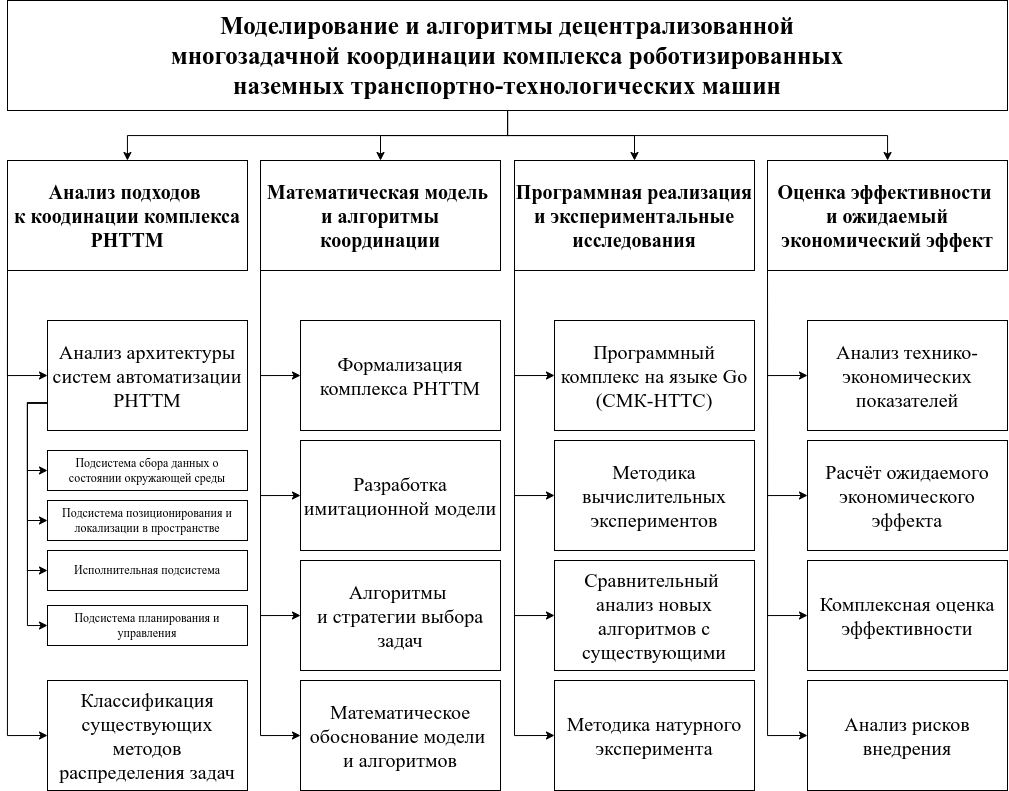
\includegraphics[scale=0.3]{scheme_diss_new.drawio.png}
    }
    \caption{Общая структура диссертационной работы}\label{fig:scheme_diss_new}
\end{figure}

\textit{Во введении} обоснована актуальность темы диссертационного исследования, сформулированы цель и задачи, определены объект и предмет исследования, представлена рабочая гипотеза, научная новизна, практическая значимость, методология и методы исследования, перечислены основные положения, выносимые на защиту, а также приведены сведения об апробации, внедрении и публикациях.

\textit{В первой главе} проведен анализ известных подходов к координации комплекса РНТТМ и методов автоматизации рабочих процессов. РНТТМ рассматриваются как высокоавтоматизированные дорожно-строительные машины (ВАЗДСМ) по ГОСТ Р 71615-2024, функционирующие на уровнях автоматизации УА2-УА5. Рассмотрены технические предпосылки реализации децентрализованной координации, включая подсистемы сбора данных, позиционирования и локализации, исполнительную подсистему, а также подсистему планирования и управления. Выполнен обзор и классификация исследований в области группового управления и распределения задач, на основе чего сформулированы цели и задачи настоящей работы.

\textit{Во второй главе} на основе данных реальных проектов строительства современных скоростных автомобильных дорог М-11 и М-12 проведена систематизация комплексов НТТМ по технологическому назначению. Это позволило сформировать репрезентативные множества машин и задач, отражающие реальные технологические комплексы и операции. Разработана имитационная модель многозадачной координации комплекса РНТТМ, учитывающая энергетические ограничения машин, неоднородность их оборудования и стохастическую природу потока задач. Предложены две новые стратегии децентрализованного выбора задач: энергосберегающая стратегия и стратегия минимизации временных задержек, формализованные на основе адаптации методов теории игр. Представлено математическое обоснование модели и алгоритмов, доказано существование байесовских равновесий Нэша и проведена оценка вычислительной сложности.

\textit{В третьей главе} осуществлена программная реализация разработанных алгоритмов на языке программирования Go, создан программный комплекс для проведения вычислительных экспериментов. Разработана методика экспериментальных исследований, включающая три сценария ресурсного обеспечения (дефицит, равновесие, избыток). Проведен сравнительный анализ предложенных стратегий с существующими подходами (прямой перебор, рыночные методы и обучение с подкреплением) на типовом комплексе и парке РНТТМ на идентичных наборах исходных данных (машин и задач). Индивидуальные характеристики каждой машины и требования каждой задачи формализованы в модели и непосредственно влияют на функцию полезности при выборе задачи, что обеспечивает объективность оценки эффективности каждой стратегии. Для количественной оценки справедливости распределения задач использован коэффициент Джини. Предложена методика проведения натурного эксперимента для верификации алгоритмов в условиях, приближенных к реальной эксплуатации.

\textit{В четвертой главе} выполнен анализ технико-экономических показателей внедрения разработанных алгоритмов децентрализованной многозадачной координации на основе синтеза результатов имитационного моделирования и данных актов внедрения. Произведен расчет ожидаемого годового экономического эффекта и срока окупаемости капитальных затрат, проведена оценка инвестиционной привлекательности. Выполнен анализ чувствительности к стоимости машино-часа и рассмотрены возможные риски внедрения, предложены меры по их минимизации.

\textit{В приложениях} приведены сводные данные по экспериментальным исследованиям, исходный код программных средств и алгоритмов, а также копии свидетельств о государственной регистрации программ для ЭВМ и актов внедрения.

\pdfbookmark{Основное содержание работы}{description}
\section*{\MakeUppercase{Основное содержание работы}}

\phantomsection
\pdfbookmark[1]{Имитационная модель координации}{sec:model}
\label{sec:model}
\par
\noindent
\textbf{1. Имитационная модель многозадачной координации комплекса РНТТМ.} Исходными данными для формализации и параметризации модели послужили утвержденные проекты организации строительства (ПОС) современных скоростных автомобильных дорог М-11 <<Москва -- Санкт-Петербург>> и М-12 <<Москва -- Нижний Новгород -- Казань>>. На основе анализа ведомостей потребности в машинах и механизмах выделены типовые технологические комплексы НТТМ: подготовительных работ, земляных работ, устройства дорожной одежды, строительства искусственных сооружений, переустройства инженерных коммуникаций и вспомогательный транспортно-технологический. Пример составов комплексов при транспортном строительстве автодорог приведен в таблицах в тексте диссертации. Каждый комплекс включает конкретные модели машин (экскаваторы ЭО-4321, ЕК-270; бульдозеры Б10ПМ, ДЗ-101А; автогрейдеры ДЗ-98; катки Hamm, Bomag; асфальтоукладчики Vogele, Titan и др.) и наборы технологических операций с нормативными показателями энергозатрат, что позволило сформировать репрезентативные множества машин и задач для имитационного моделирования.

На рис.~\ref{fig:sensors} представлена принципиальная схема РНТТМ как элемента множества. Схема отражает архитектуру бортовой системы управления, включающую сенсорные подсистемы, вычислительный блок с реализованными алгоритмами принятия решений, каналы связи с другими машинами, диспетчерским центром и исполнительными механизмами.

\begin{figure}[ht]
    \centering{
        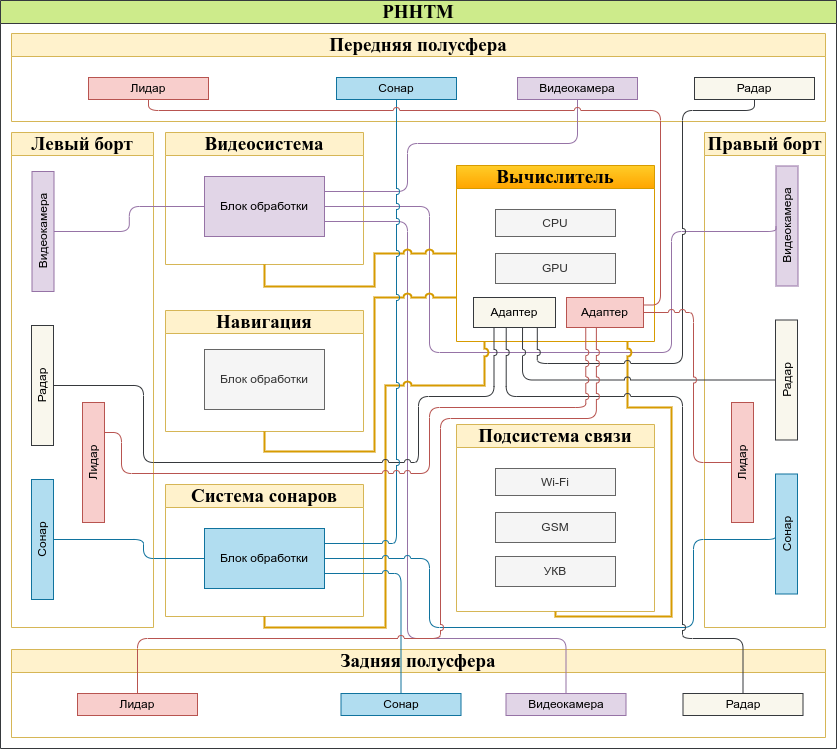
\includegraphics[scale=0.3]{tech.drawio.png}
    }
    \caption{Принципиальная схема РНТТМ}\label{fig:sensors}
\end{figure}

В основу модели (рис. \ref{fig:system_model}) положено представление комплекса РНТТМ как множества машин $ R_i $ ($ i = 1,\dots,N $), каждая из которых характеризуется набором технологического оборудования $ \text{Eq}_i $ (ковш, отвал, вибровалец и т.д.) и запасом энергии $ E_i \in [0, E_{\max}] $. Динамика энергии описывается соотношением
\begin{equation}
E_i(t + \Delta t) = \min\left\{\max\left\{E_i(t) - e_{T_j} \cdot \mathbf{1}(A_i = T_j) + r_i \Delta t,\; 0\right\},\; E_{\max}\right\},
\end{equation}
где $E_i(t)$ и $E_i(t + \Delta t)$ -- запас энергии $i$-й РНТТМ в момент времени $t$ и $t+\Delta t$ соответственно; $\Delta t$ -- шаг дискретизации; $e_{T_j}$ -- энергозатраты на выполнение $j$-й задачи; $A_i$ -- действие $i$-й РНТТМ (выбор задачи $T_j$); $\mathbf{1}(A_i = T_j)$ -- индикаторная функция, принимающая значение 1, если $i$-я РНТТМ выбрала задачу $T_j$, и 0 в противном случае; $r_i$ -- скорость восстановления ресурса $i$-й РНТТМ; $E_{\max}$ -- максимальный запас энергии. Поток задач $ \mathcal{T}(t) = \{T_1,\dots,T_{M(t)}\} $ формируется двумя независимыми пуассоновскими процессами (внешним и внутренним) с суммарной интенсивностью $ \lambda = \lambda_s + \lambda_l $. Каждая задача $ T_j $ характеризуется сложностью $ \Theta_{T_j} $, распределенной по усеченному нормальному закону $ \mathcal{N}_{[0,+\infty)}(\mu_T, \sigma_T^2) $, и требуемым типом оборудования $ \text{Req}_j $.

\begin{figure}[ht!]
    \centering{
        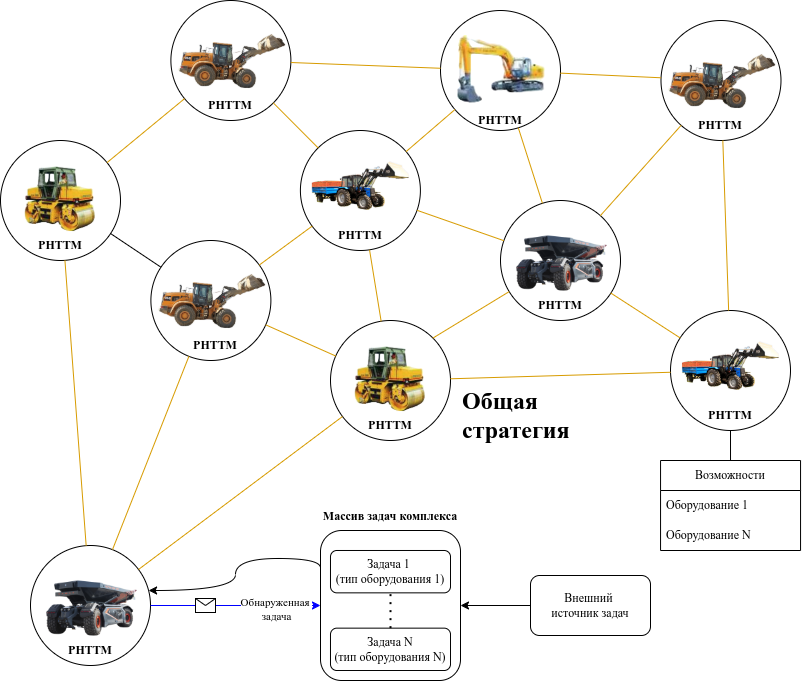
\includegraphics[scale=0.35]{system-math.drawio.png}
    }
    \caption{Граф взаимодействия системы многозадачной координации комплекса РНТТМ}\label{fig:system_model}
\end{figure}

Предлагаемая имитационная модель построена на следующих основных допущениях:
\begin{itemize}[beginpenalty=10000, midpenalty=10000, wide=\parindent, leftmargin=0pt]
    \item поток задач является пуассоновским, а сложность каждой задачи распределена по усеченному нормальному закону;
    \item энергопотребление при выполнении задачи детерминировано и линейно зависит от ее сложности, время выполнения пропорционально этой сложности;
    \item каждая машина может выполнять только те задачи, для которых ее навесное оборудование удовлетворяет требованиям задачи;
    \item взаимодействие между машинами осуществляется по фиксированному связному неориентированному графу, решения принимаются дискретно во времени синхронно;
    \item влияние рабочей среды на эффективность работы машин в явном виде не учитываются. Предполагается, что эти факторы уже отражены в детерминированных и статистически заданных параметрах сложности задач;
    \item вся необходимая для выбора задачи информация (сложность, требуемое оборудование, уровень энергии) считается достоверной и доступной локально.
\end{itemize}

Так как объектом исследования является \textbf{системный уровень координации} комплекса машин, а именно распределение задач и децентрализованное принятие решений, то взаимодействие с рабочей средой считается заданным на нижнем уровне автоматизации (штатные системы управления рабочим органом) и не влияет напрямую на предлагаемые далее алгоритмы координации, за исключением энергозатрат \( \Theta_{T_j} \), которые являются входным параметром модели. Математические модели физического взаимодействия РНТТМ с рабочей средой (грунтом, дорожным покрытием) не рассматриваются в работе. Управление рабочими органами, стабилизация движения и другие задачи нижнего уровня автоматизации считаются штатно решенными и не являются предметом моделирования. На уровне принятия решений о распределении задач влияние среды считается постоянным в пределах одного эксперимента.

Задача доступна машине при одновременном выполнении условий совместимости оборудования и достаточности энергии:
\begin{equation}
\mathcal{T}_i(t) = \{T_j \in \mathcal{T}(t) \mid \text{Eq}_i \succeq \text{Req}_j,\; E_i \ge \Theta_{T_j}\},
\end{equation}
где $\mathcal{T}_i(t)$ -- локальный массив задач, доступных $i$-й РНТТМ в момент времени $t$; $\mathcal{T}(t)$ -- общий групповой массив задач; $T_j$ -- $j$-я задача; $\text{Eq}_i$ -- набор оборудования $i$-й РНТТМ; $\text{Req}_j$ -- требуемый тип оборудования для выполнения задачи $T_j$; запись $ \text{Eq}_i \succeq \text{Req}_j $ означает, что набор оборудования машины $ \text{Eq}_i $ удовлетворяет или превосходит требования задачи $ \text{Req}_j $; $E_i$ -- текущий запас энергии $i$-й РНТТМ; $ \Theta_{T_j} $ -- требуемый объем энергозатрат (сложность) на выполнение задачи $ T_j $.

Взаимодействие машин моделируется связным неориентированным графом $ G = ([N], \mathcal{E}) $; множество соседей машины $ R_i $ обозначается $ \mathcal{R}_i $. Каждая РНТТМ выбирает задачу в соответствии со стратегией $ \gamma_i $, а профиль стратегий всего комплекса есть $ \Gamma = (\gamma_1,\dots,\gamma_N) $. Поведение комплекса описывается координационной игрой с локальной функцией полезности вида:
\begin{equation}
    V_i(\mathbf{A},\Theta) \equiv \sum_{j \in \mathcal{R}_i} \alpha \cdot \mathbf{1}(A_i = A_j) - \beta \Theta(A_i),
\end{equation}
где $V_i(\mathbf{A},\Theta)$ -- функция полезности $i$-й РНТТМ; $\mathbf{A} = (A_1, \dots, A_N)$ -- вектор действий всех РНТТМ комплекса; $\Theta$ -- вектор сложностей задач; $A_i$ и $A_j$ -- действия $i$-й и $j$-й РНТТМ соответственно; $\mathcal{R}_i$ -- множество соседей $i$-й РНТТМ в графе взаимодействий; $\mathbf{1}(A_i = A_j)$ -- индикаторная функция, равная 1, если соседи выбрали одну задачу, и 0 в противном случае; $\alpha > 0$ -- коэффициент поощрения (выигрыш) за координацию; $\beta > 0$ -- штрафной коэффициент за сложность; $\Theta(A_i)$ -- сложность задачи, выбранной $i$-й РНТТМ. Стратегия $\gamma^* = (\gamma_1^*,\dots,\gamma_N^*)$ является байесовским равновесием Нэша, если для каждой $i$-й РНТТМ выполняется условие:
\begin{equation}
    J_i(\gamma_i^*, \gamma_{-i}^*) \ge J_i(\gamma_i, \gamma_{-i}^*), \quad \gamma_i \in \Gamma_i, \forall i \in [N],
\end{equation}
где $J_i$ -- ожидаемый выигрыш $i$-й РНТТМ; $\gamma_i^*$ -- оптимальная стратегия $i$-й РНТТМ; $\gamma_{-i}^*$ -- профиль стратегий всех остальных РНТТМ комплекса; $\gamma_i$ -- любая альтернативная стратегия $i$-й РНТТМ; $\Gamma_i$ -- множество допустимых стратегий $i$-й РНТТМ; $[N]$ -- множество всех РНТТМ в комплексе. Доказано существование таких равновесий, зависящих от структуры графа и соотношения сложностей задач.

Выполнено сопоставление предложенной модели с классической системой массового обслуживания; показано, что в отличие от стандартных подходов, разработанная модель учитывает неоднородность машин, стохастическую сложность задач и децентрализованный характер принятия решений, что обеспечивает ее адекватность реальным условиям эксплуатации.

\FloatBarrier

\phantomsection
\pdfbookmark[1]{Алгоритмы децентрализованной координации}{sec:algo}
\label{sec:algo}

\textbf{2. Алгоритмы децентрализованной многозадачной координации комплекса РНТТМ.} С использованием предложенной модели формализованы две новые стратегии децентрализованного выбора задач:
\begin{itemize}[beginpenalty=10000, midpenalty=10000, wide=\parindent, leftmargin=0pt]
    \item \textit{Энергосберегающая стратегия} $ \Gamma_{\min\text{Э}} $ (рис. \ref{fig:algo}), в которой функция полезности $ i $-й машины имеет вид
    \begin{equation}
        \mathcal{V}_i^{\min\text{Э}}(\mathbf{A}, \Theta, E_i) = \alpha \sum_{j \in \mathcal{R}_i}
        \mathbf{1}(A_i = A_j) - \beta \frac{\Theta_{A_i}}{E_i},
    \end{equation}
    где $\mathcal{V}_i^{\min\text{Э}}$ -- функция полезности энергосберегающей стратегии для $i$-й РНТТМ; $\mathbf{A}$ -- вектор действий всех машин комплекса; $\Theta$ -- вектор сложностей задач; $E_i$ -- текущий запас энергии $i$-й РНТТМ; $\mathcal{R}_i$ -- множество соседей машины $R_i$ в графе взаимодействий; $\mathbf{1}(A_i = A_j)$ -- индикаторная функция совпадения действий соседей; $\alpha > 0$ -- коэффициент поощрения за скоординированный выбор одной и той же задачи с соседями; $\beta > 0$ -- штрафной коэффициент; $\Theta_{A_i}$ -- сложность задачи, выбранной $ i $-й машиной. Второе слагаемое $ \beta \Theta_{A_i}/E_i $ представляет собой энергоэффективность задачи, что позволяет каждой машине автономно минимизировать отношение затрат к оставшемуся ресурсу.

    \item \textit{Стратегия минимизации временных задержек}
    $ \Gamma_{\min\text{ВЗ}} $ (рис. \ref{fig:algo2}), вводящая динамику времени ожидания задачи $ W_j $, которая описывается соотношением:
    \begin{equation}
        W_j(t + \Delta t) = \begin{cases} 0 & \text{при выполнении,} \\ W_j(t) \cdot e^{\lambda \Delta t} & \text{иначе,} \end{cases}
    \end{equation}
    где $W_j(t)$ и $W_j(t + \Delta t)$ -- время ожидания $j$-й задачи в очереди в момент времени $t$ и $t+\Delta t$ соответственно; $\Delta t$ -- шаг дискретизации; $\lambda > 0$ -- коэффициент роста задержки во времени. Целевая функция $i$-й РНТТМ имеет вид:
    \begin{equation}
        \mathcal{V}_i^{\min\text{ВЗ}}(\mathbf{A}, \Theta) = -\beta W_{A_i}(t) \Theta_{A_i} +
        \alpha \sum_{j \in \mathcal{R}_i} \mathbf{1}(A_i = A_j),
    \end{equation}
    где $\mathcal{V}_i^{\min\text{ВЗ}}$ -- функция полезности стратегии минимизации временных задержек; $\mathbf{A}$ -- вектор действий; $\Theta$ -- вектор сложностей задач; $\beta$ -- штрафной коэффициент; $W_{A_i}(t)$ -- время нахождения задачи, выбранной $i$-й РНТТМ, в очереди; $\Theta_{A_i}$ -- сложность выбранной задачи; $\alpha$ -- коэффициент поощрения; $\mathcal{R}_i$ -- множество соседей; $\mathbf{1}(A_i = A_j)$ -- индикаторная функция совпадения действий. Первое слагаемое $ -\beta W_{A_i}(t) \Theta_{A_i} $ формирует штраф, пропорциональный как сложности задачи, так и длительности ее ожидания, что заставляет комплекс отдавать приоритет <<стареющим>> задачам и предотвращать неограниченный рост задержек.
\end{itemize}

Для разработанных стратегий выполнено математическое обоснование: доказано существование по крайней мере одного байесовского равновесия Нэша. Например, для энергосберегающей стратегии равновесие достигается при:
\begin{equation}
    A_i^* = \min_{k \in \mathcal{T}_i(t)} \left( \frac{\Theta_k}{E_i} - \frac{\alpha}{\beta} \cdot \mathbb{E}\left[|\{j \in \mathcal{R}_i : A_j = k\}|\right] \right),
\end{equation}
где $A_i^*$ -- оптимальное действие (выбор задачи) $i$-й РНТТМ при достижении равновесия; $k$ -- индекс рассматриваемой задачи из локального массива $\mathcal{T}_i(t)$; $\Theta_k$ -- сложность $k$-й задачи; $E_i$ -- текущий запас энергии $i$-й РНТТМ; $\alpha$ и $\beta$ -- весовые коэффициенты поощрения и штрафа; $\mathbb{E}[\cdot]$ -- математическое ожидание; $|\{j \in \mathcal{R}_i : A_j = k\}|$ -- мощность множества соседей $i$-й РНТТМ, выбравших ту же задачу $k$.

\begin{figure}[H]
    \centering{
        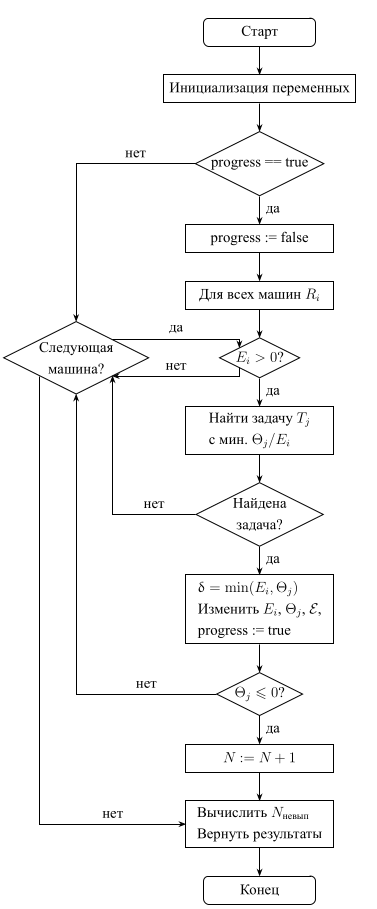
\includegraphics[scale=0.48]{algo.png}
    }
    \caption{Алгоритм энергосберегающей стратегии децентрализованной многозадачной координации комплекса РНТТМ}\label{fig:algo}
\end{figure}

% Первая часть алгоритма
\begin{figure}[H]
    % \centering
    \subcaptionbox{Начало\label{fig:algo_part1}}{%
        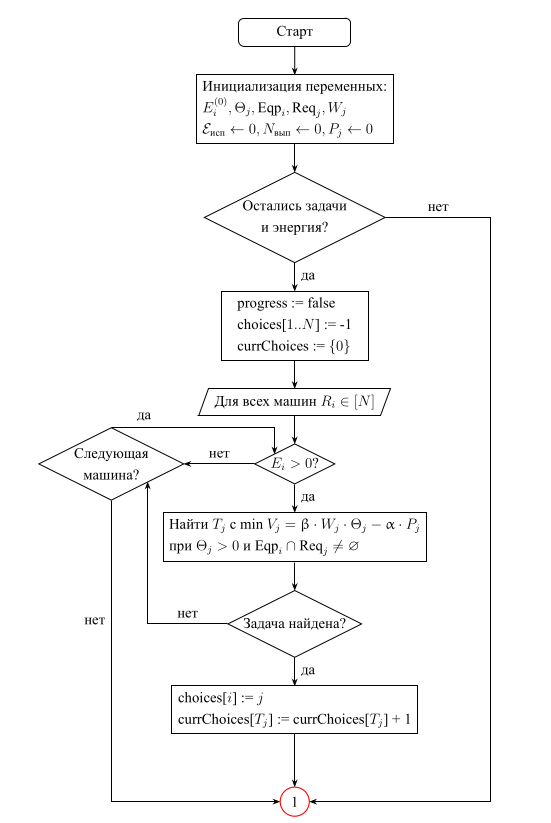
\includegraphics[scale=0.48]{algo_2_1.png}%
    }
    % Основная подпись с правильным разделителем и без точки в конце
    \caption{Алгоритм стратегии минимизации временных задержек децентрализованной многозадачной координации комплекса РНТТМ}%
    \label{fig:algo2}
\end{figure}

% Вторая часть алгоритма (продолжение)
\begin{figure}[H]
    \ContinuedFloat % <-- ОБЯЗАТЕЛЬНО! Продолжает нумерацию рисунка
    \centering
    \subcaptionbox{Окончание\label{fig:algo_part2}}{%
        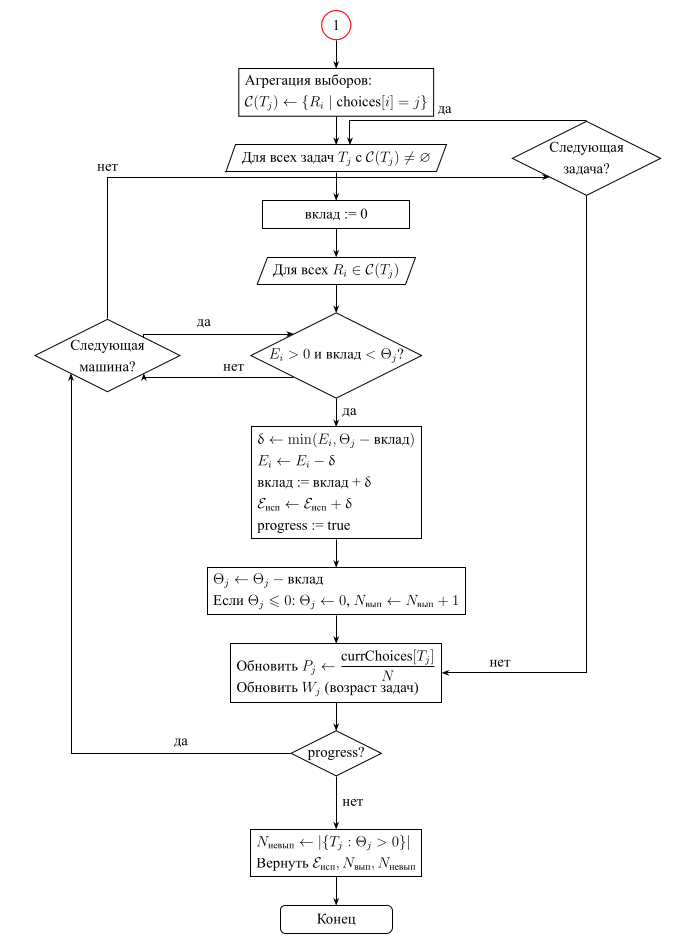
\includegraphics[scale=0.45]{algo_2_2.png}%
    }
    % Подпись для продолжения. Здесь можно дать краткое пояснение.
    \caption{Алгоритм стратегии минимизации временных задержек децентрализованной многозадачной координации комплекса РНТТМ}%
    \label{fig:algo_cont}
\end{figure}

Установлена сходимость алгоритмов за конечное число итераций и получена оценка вычислительной сложности:
\begin{equation}
    \mathcal{O}(N \cdot M \cdot \Delta), \text{ где } \Delta = \max_i |\mathcal{R}_i|,
\end{equation}
где $\mathcal{O}(\cdot)$ -- асимптотическая оценка вычислительной сложности; $N$ -- количество РНТТМ в комплексе; $M$ -- количество доступных задач в системе; $\Delta$ -- максимальная степень вершины в графе взаимодействий (максимальное число соседей у одной РНТТМ). Полученная оценка существенно эффективнее полного перебора ($ \mathcal{O}(M^N) $). Проведен анализ устойчивости решений к малым возмущениям параметров, показывающий, что формализация выбора задач в терминах байесовского равновесия обеспечивает устойчивость распределения при неполной информации о состоянии частей комплекса РНТТМ.

\FloatBarrier

\phantomsection
\pdfbookmark[1]{Результаты экспериментальных исследований c комплексной оценкой эффективности разработанных алгоритмов}{sec:results}
\label{sec:results}

\textbf{3. Результаты экспериментальных исследований c комплексной оценкой эффективности разработанных алгоритмов.} Программная реализация разработанных алгоритмов выполнена на языке Go. Создана платформа моделирования, обеспечивающая проведение вычислительных экспериментов для комплексов различной численности в контролируемых условиях. Разработаны методики проведения вычислительных экспериментов с использованием программной платформы и проведения натурного эксперимента.

Архитектура программного комплекса построена по модульному принципу (рис. \ref{fig:program_modules}) и включает: модуль конфигураций, модуль моделей и модуль стратегий, в который подгружаются наборы стратегий координации, реализующих общий интерфейс. Главный исполняемый файл импортирует эти модули, осуществляет прогон симуляций по стратегиям на единых исходных данных конфигураций и моделях машин и задач с формированием отчетов и последующим их анализом. Такой подход обеспечивает гибкость и расширяемость системы, позволяя добавлять новые алгоритмы и сравнивать их в единой среде. Ключевые компоненты реализованы с использованием встроенных механизмов конкурентности Go (горутины, каналы), что адекватно отражает децентрализованный характер взаимодействия РНТТМ.

\begin{figure}[h!]
    \centering{
        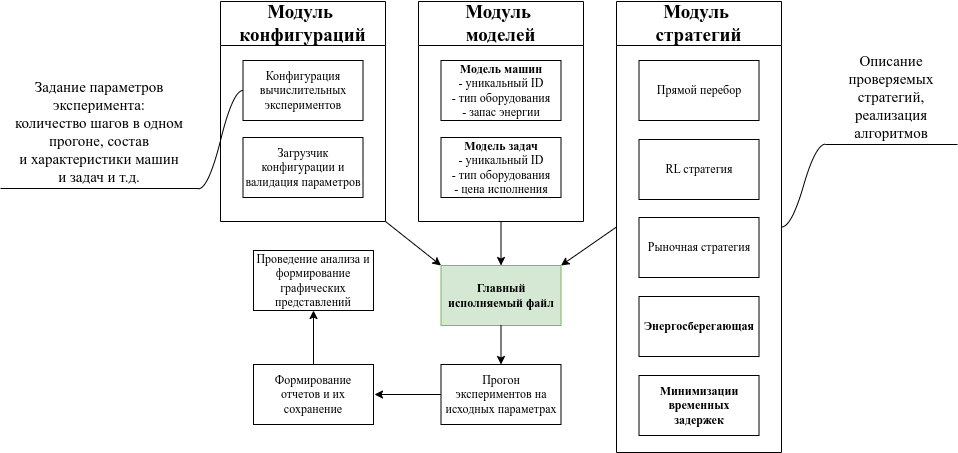
\includegraphics[scale=0.34]{programm.drawio.png}
    }
    \caption{Модульная структура программного средства СМК-НТТС}
    \label{fig:program_modules}
\end{figure}

В платформе реализованы пять стратегий распределения задач: две разработанные автором (энергосберегающая $ \Gamma_{\min\text{Э}} $ и минимизации временных задержек $ \Gamma_{\min\text{ВЗ}} $) и три сравнительных (прямой перебор, рыночный метод, Q-обучение). На программные средства получены свидетельства о государственной регистрации программ для ЭВМ.

Методика экспериментов включает три сценария, моделирующих различное соотношение суммарной энергии машин и энергоемкости задач: дефицитный ($ \sum E_i = 0{,}5 \sum \Theta_j $), равновесный ($ \sum E_i = \sum \Theta_j $) и избыточный ($ \sum E_i = 2 \sum \Theta_j $). Для обеспечения статистической достоверности каждый эксперимент проводился с $ N $ независимыми прогонами на идентичных исходных данных. В качестве ключевых метрик использовались: количество выполненных задач, суммарные энергозатраты, общее время выполнения, средние и медианные значения, а также коэффициент Джини $ G(\mathbf{x}) $ для количественной оценки справедливости распределения нагрузки:
\begin{equation}
    G(\mathbf{x}) = \frac{\sum_{i=1}^N \sum_{j=1}^N |x_i - x_j|}{2N \sum_{i=1}^N x_i}.
\end{equation}
где $G(\mathbf{x})$ -- коэффициент Джини; $\mathbf{x} = (x_1, \dots, x_N)$ -- вектор распределения ресурса (нагрузки) между $N$ машинами; $x_i$ и $x_j$ -- значения нагрузки (например, количества выполненных задач или затраченной энергии) $i$-й и $j$-й РНТТМ соответственно; $N$ -- количество РНТТМ в комплексе.

Таким образом, разработанная имитационная модель многозадачной децентрализованной координации комплекса РНТТМ позволила провести вычислительные эксперименты, используя следующие принципы теории:
\begin{itemize}[beginpenalty=10000, midpenalty=10000, wide=\parindent, leftmargin=0pt]
    \item \textbf{контролируемые сценарии} -- три уровня ресурсного обеспечения (дефицит, равновесие, избыток);
    \item \textbf{многократные повторения} -- каждая стратегия прогоняется \( R = 30 \) раз в каждом сценарии;
    \item \textbf{закон больших чисел} -- выборочные средние метрик сходятся к истинному математическому ожиданию при увеличении числа прогонов;
    \item \textbf{коэффициент Джини} \( G(\mathbf{x}) \) -- для количественной оценки справедливости распределения нагрузки между машинами;
    \item \textbf{анализ чувствительности} -- варьирование стоимости машино-часа \( C_{\text{мч}} \) в диапазоне 500-5000 руб./ч для оценки устойчивости экономических показателей.
\end{itemize}

Вычислительные эксперименты проведены для двух конфигураций, сформированных на основе данных проектов организации строительства современных автодорог М-11 и М-12:
\begin{itemize}[beginpenalty=10000, midpenalty=10000, wide=\parindent, leftmargin=0pt]
    \item \textit{типовой комплекс}~-- 15 РНТТМ (экскаваторы, бульдозеры, автогрейдеры, катки, асфальтоукладчик, фреза, автогудронатор, буровая машина, автокран), соответствующий специализированному комплексу по возведению земляного полотна и устройству дорожной одежды;
    \item \textit{парк машин}~-- 100 РНТТМ, отражающий суммарный парк техники для нескольких технологических потоков при строительстве скоростной автомобильной дороги (перечень приведен в тексте работы).
\end{itemize}

Основные результаты:
\begin{itemize}[beginpenalty=10000, midpenalty=10000, wide=\parindent, leftmargin=0pt]
    \item в сценарии дефицита ресурсов (рис. \ref{fig:result_1} и \ref{fig:result_2}) энергосберегающая стратегия $ \Gamma_{\min\text{Э}} $ выполнила $ 51{,}6\,\% $ задач (типовой комплекс) и $ 50{,}5\,\% $ (парк машин), что в $ 1{,}4 $--$ 1{,}5 $ раза превышает показатели сравнительных методов ($ 36{,}2\,\% $ и $ 37{,}7\,\% $ соответственно);
    \item в равновесном и избыточном сценариях $ \Gamma_{\min\text{Э}} $ также демонстрирует наилучшие или сопоставимые с лучшими результаты, обеспечивая при этом максимальную энергоэффективность (минимальные затраты на задачу);
    \item стратегия $ \Gamma_{\min\text{Э}} $ обладает наилучшим балансом между эффективностью и скоростью выполнения: ее время работы значительно ниже, чем у Q-обучения, и сопоставимо с рыночными методами;
    \item анализ коэффициента $ G(\mathbf{x}) $ подтвердил, что энергосберегающая стратегия обеспечивает не только высокую производительность, но и статистически справедливое распределение нагрузки между машинами. Интегральная оценка эффективности, рассчитанная как:
    \begin{equation}
        \begin{split}
        Q(\Gamma) = \alpha_1 \tilde{P}(\Gamma) + \alpha_2 \tilde{\eta}(\Gamma) + \alpha_3 (1 - \tilde{T}(\Gamma)) + \\
        + \alpha_4 (1 - G^{\text{задачи}}) + \alpha_5 (1 - G^{\text{энергии}}),
        \end{split}
    \end{equation}
    где $Q(\Gamma)$ -- интегральная оценка эффективности стратегии $\Gamma$; $\alpha_1, \dots, \alpha_5$ -- весовые коэффициенты, удовлетворяющие условию $\sum_{i=1}^5 \alpha_i = 1$; $\tilde{P}(\Gamma)$ -- нормализованное значение процента выполнения задач; $\tilde{\eta}(\Gamma)$ -- нормализованный коэффициент энергоэффективности; $\tilde{T}(\Gamma)$ -- нормализованное общее время выполнения; $G^{\text{задачи}}$ и $G^{\text{энергии}}$ -- коэффициенты Джини для распределения количества задач и энергозатрат соответственно. Интегральная оценка составила $ Q = 0{,}84 $ для $\Gamma_{\min\text{Э}}$ против $ 0{,}52 $--$ 0{,}79 $ у других методов.
\end{itemize}

\begin{figure}[ht!]
    \centering{
        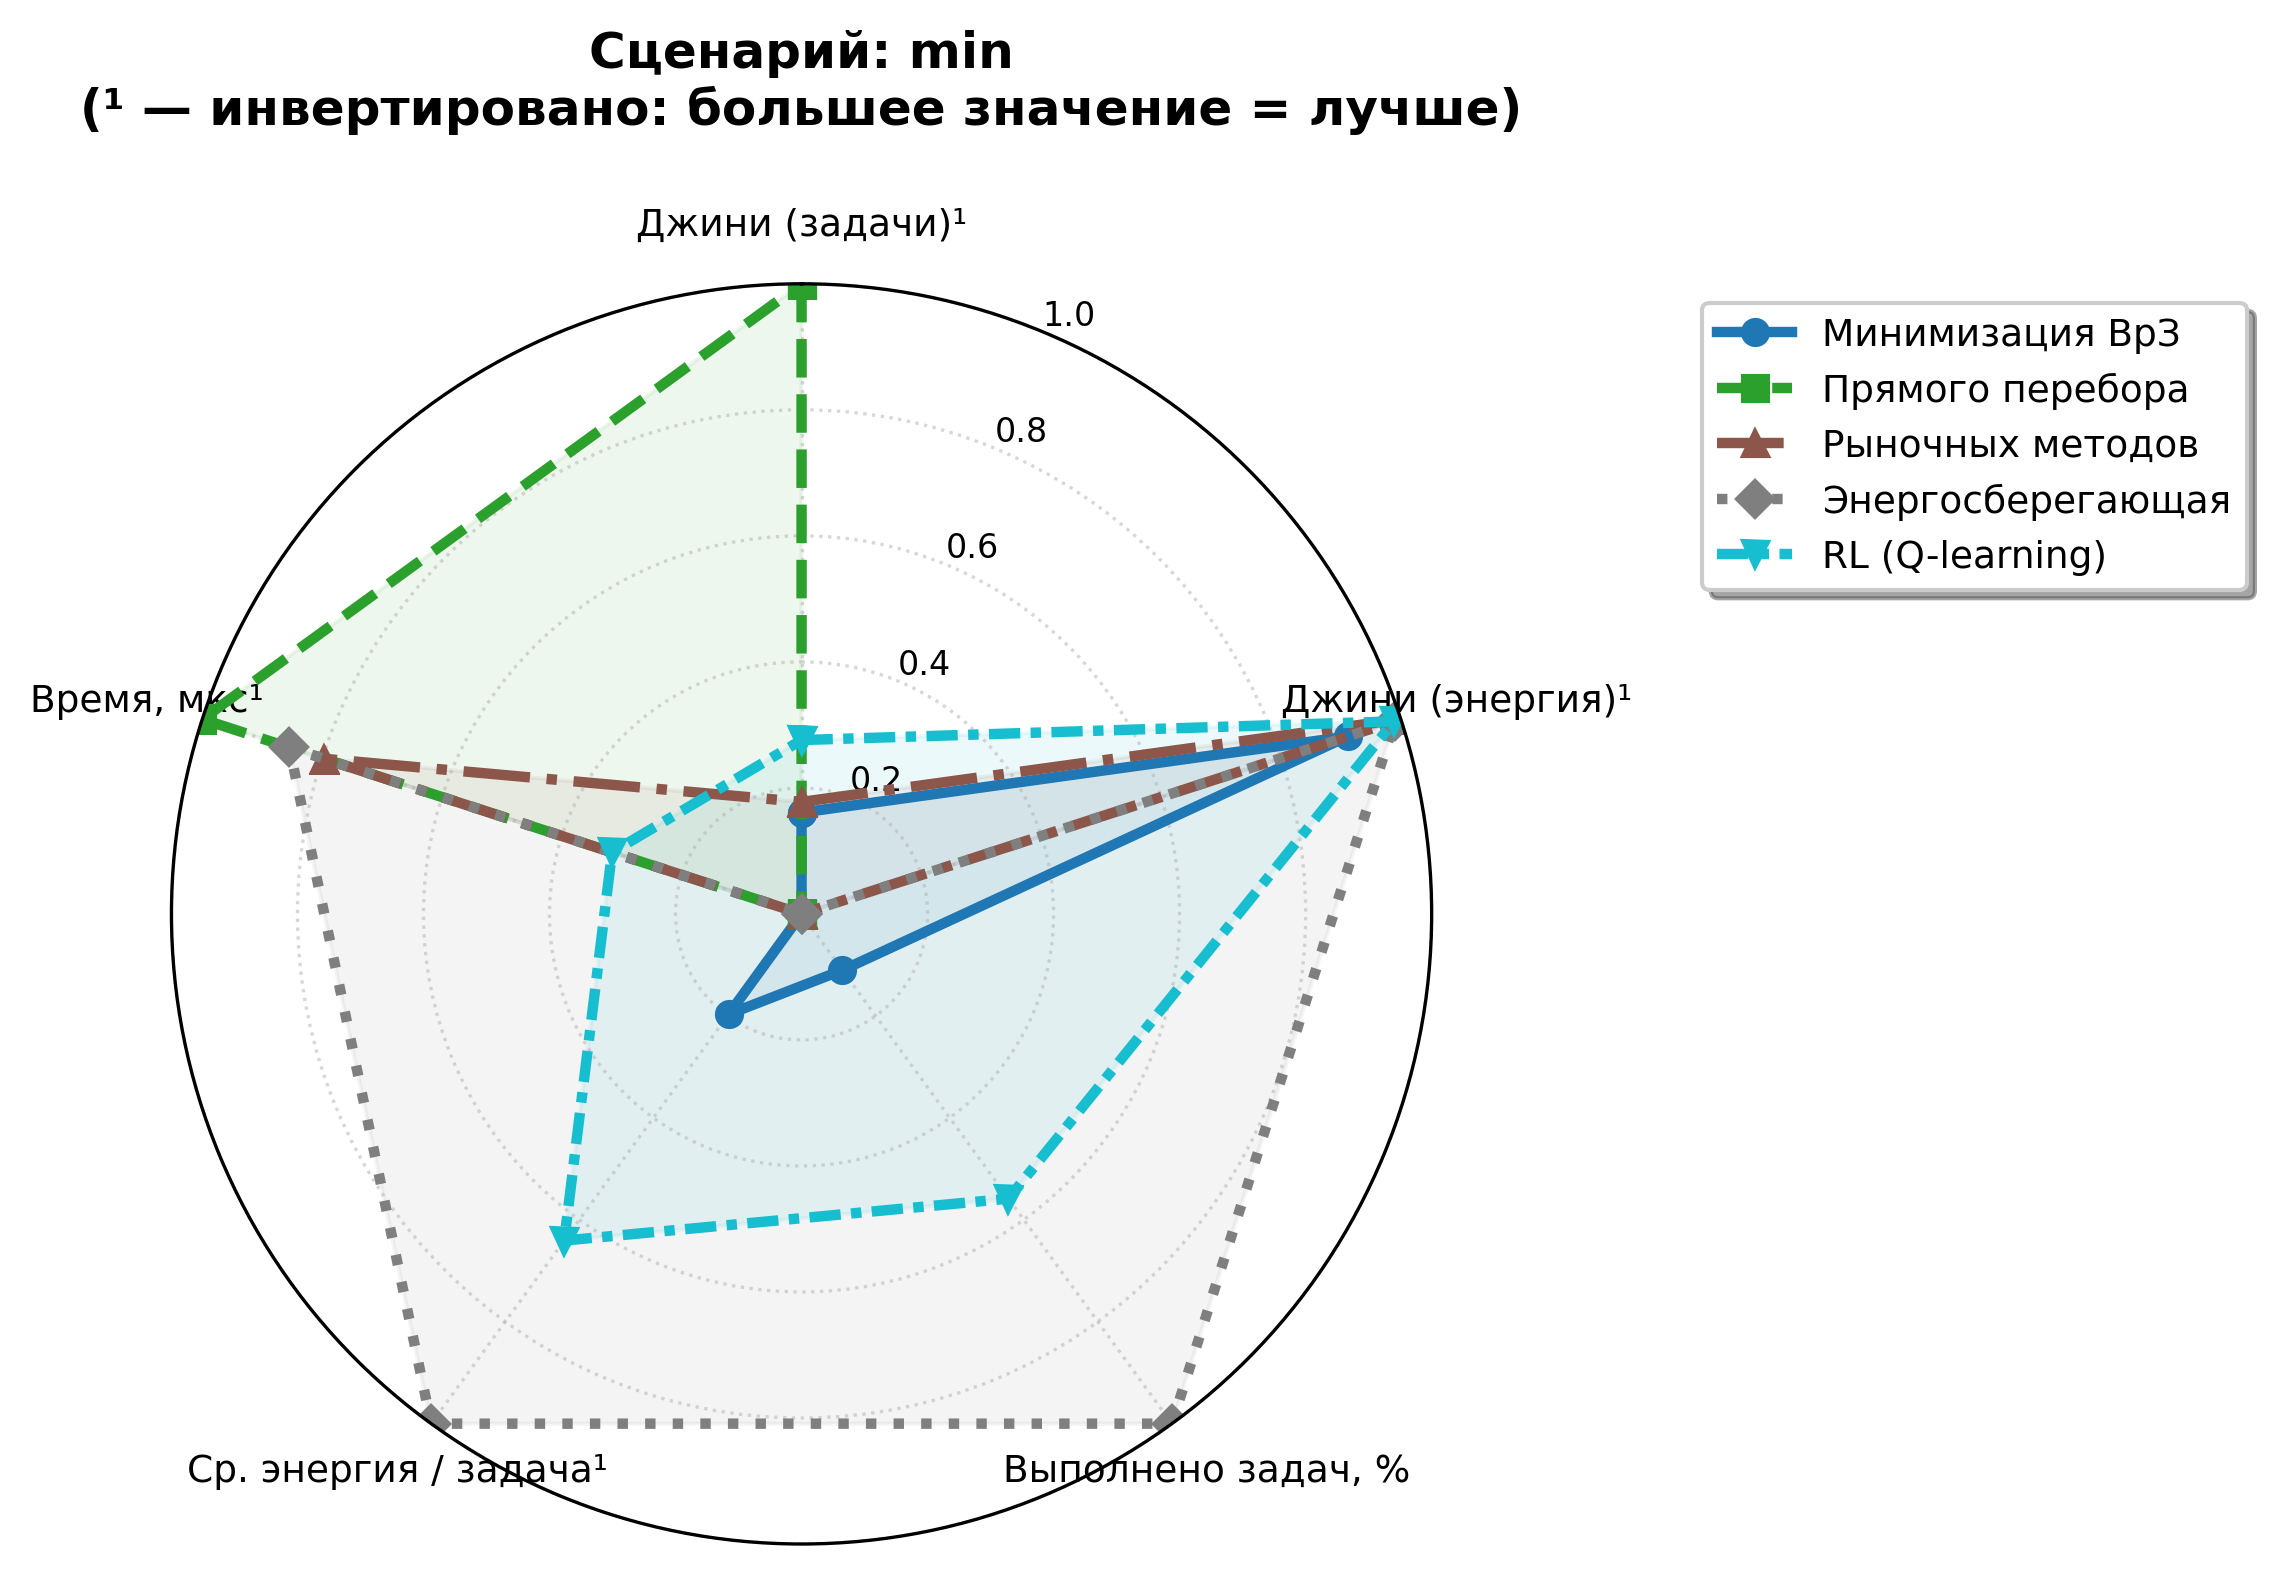
\includegraphics[scale=0.45]{radar_min_8.png}
    }
    \caption{Круговая диаграмма значений дефицитного сценария эксперимента для типового комплекса РНТТМ}\label{fig:result_1}
\end{figure}

\begin{figure}[ht!]
    \centering{
        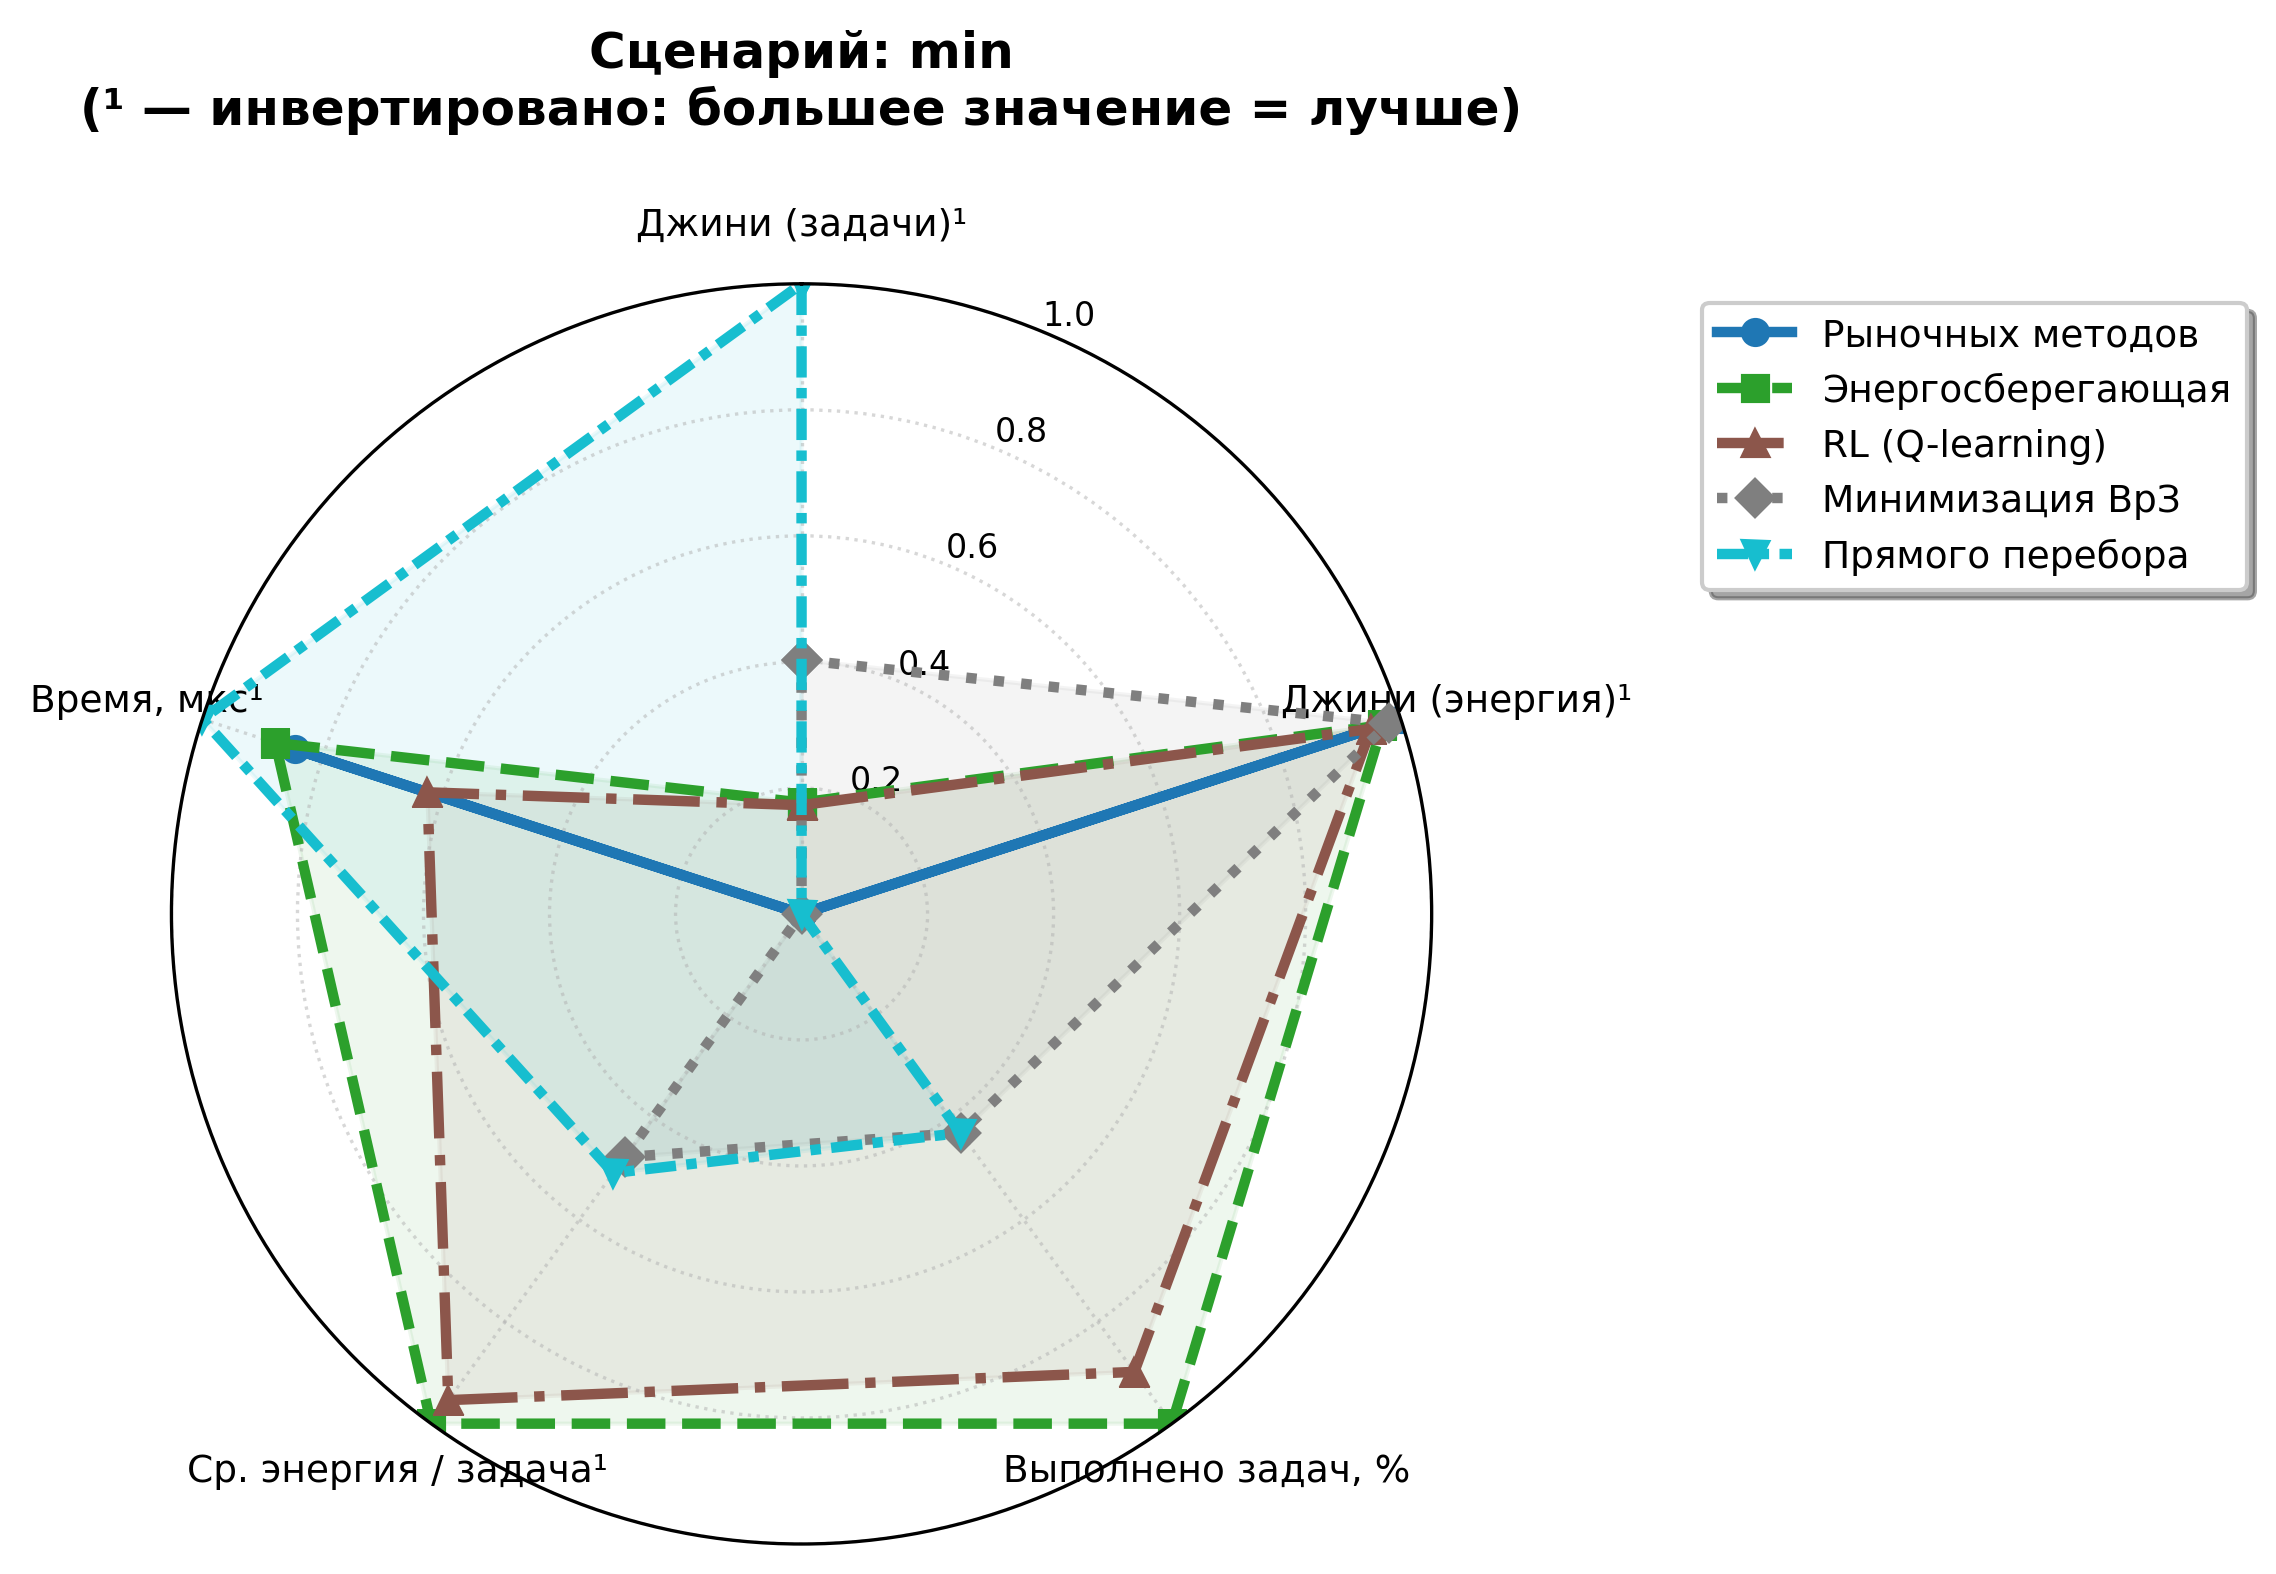
\includegraphics[scale=0.45]{radar_min_100.png}
    }
    \caption{Круговая диаграмма значений дефицитного сценария эксперимента для парка РНТТМ}\label{fig:result_2}
\end{figure}

Практическое внедрение стратегии $ \Gamma_{\min\text{Э}} $ подтвердило основные тенденции, предсказанные теоретической моделью. Согласно актам внедрения, применение разработанных алгоритмов обеспечило:
\begin{itemize}[beginpenalty=10000, midpenalty=10000, wide=\parindent, leftmargin=0pt]
    \item рост производительности комплекса РНТТМ на $ 11{,}2 $-$ 13{,}1\,\% $;
    \item сокращение общего времени выполнения операций на $ 8{,}7 $-$ 9{,}1\,\% $;
    \item повышение энергоэффективности (снижение удельных энергозатрат) на $ 11{,}8 $-$ 12{,}3\,\% $;
    \item уменьшение времени простоев оборудования на $ 8{,}2 $-$ 9{,}1\,\% $.
\end{itemize}

Ожидаемый экономический эффект формируется преимущественно за счет экономии машино-часов. При годовом фонде времени эксплуатации комплекса из 10 машин $ T_{\text{год}} = 20\,000 $ машино-часов и подтвержденной экономии времени $ 8{,}9\,\% $ годовая экономия составляет $ \Delta T_{\text{год}} = 1\,780 $ машино-часов. При консервативной оценке стоимости машино-часа $ C_{\text{мч}} = 1\,500 $ руб./ч годовой экономический эффект равен:
\begin{equation}
E_{\text{год}} = \Delta T_{\text{год}} \cdot C_{\text{мч}} = 1\,780 \cdot 1\,500 = 2{,}67 \text{ млн руб.}
\end{equation}
где $E_{\text{год}}$ -- годовой экономический эффект, млн руб.; $\Delta T_{\text{год}}$ -- годовая экономия времени эксплуатации, машино-ч; $C_{\text{мч}}$ -- стоимость одного машино-часа, руб./ч.

Капитальные затраты на внедрение (адаптация программного обеспечения, обучение персонала) оценены в $ K = 4{,}5 $ млн руб. Срок окупаемости:
\begin{equation}
T_{\text{ок}} = \frac{K}{E_{\text{год}}} = \frac{4{,}5}{2{,}67} \approx 1{,}7 \text{ года}.
\end{equation}
где $T_{\text{ок}}$ -- срок окупаемости капитальных вложений, лет; $K$ -- капитальные затраты на внедрение, млн руб.; $E_{\text{год}}$ -- годовой экономический эффект, млн руб.

Проведен анализ чувствительности для различных значений $ C_{\text{мч}} $ (от 500 до 5 000 руб./ч), подтвердивший инвестиционную привлекательность разработки во всем диапазоне, характерном для дорожно-строительной и специальной техники.

Качественные преимущества внедрения стратегии $ \Gamma_{\min\text{Э}} $ включают: повышение отказоустойчивости системы за счет децентрализованной архитектуры, снижение влияния человеческого фактора, адаптивность к изменению состава задач и внешних условий.

Рассмотрены и систематизированы потенциальные риски (технические, организационные, эксплуатационные, экономические) и предложены меры их минимизации.

\pdfbookmark{Заключение}{conclusion}                                  % Закладка pdf
\section*{\MakeUppercase{Заключение}}
\label{sec:all_result}
В \underline{\textbf{заключении}} приведены основные результаты работы:
%% Согласно ГОСТ Р 7.0.11-2011:
%% 5.3.3 В заключении диссертации излагают итоги выполненного исследования, рекомендации, перспективы дальнейшей разработки темы.
%% 9.2.3 В заключении автореферата диссертации излагают итоги данного исследования, рекомендации и перспективы дальнейшей разработки темы.
\begin{enumerate}
	\item На основе анализа существующих подходов к распределению и~координации задач в группах роботизированных наземных транспортно-технологических средств сформулирована формальная модель многозадачной координации, учитывающая ограничения по энергии, оборудование машин и стохастичность появления задач.
	\item Численные исследования показали, что предложенная \emph{энергосберегаю-щая стратегия} обеспечивает наилучшее соотношение <<выполненные задачи / потраченная энергия>> во всех исследованных сценариях: обеспечивается максимальная эффективность выполнения задач, лучшая адаптивность при ограниченных ресурсах и устойчивость результатов по сравнению с другими методами. По времени выполнения сохраняются приемлемые показатели, а в практических сценариях рекомендуется для промышленного внедрения.
	\item Математическое моделирование (аналитическая оценка <<цен игр>> для предложенных стратегий и численная проверка на серии статистически контролируемых экспериментов) продемонстрировало, что выбор оптимальной стратегии зависит от начальных распределений энергоресурсов, статистики сложности задач и динамики веса при формировании приоритетов задач; в большинстве практических распределений выигрывает энергосберегающая стратегия. Методология моделирования и критерии сравнения (время, энергия, стабильность) подробно описаны и верифицированы.
	\item Для выполнения поставленных задач был создан программный комплекс на языке Go: реализованы модели машин и задач, набор стратегий (энергосберегающая, минимизации задержек, прямой перебор, рыночные методы, RL/Q-learning), модуль запуска экспериментов и~модуль анализа/генерации графиков и отчётов. Описаны экспериментальная среда и сценарии тестирования, представлены результаты экспериментов.
\end{enumerate}


% \clearpage

\pdfbookmark{Литература}{bibliography}                                % Закладка pdf
% При использовании пакета \verb!biblatex! список публикаций автора по теме
% диссертации формируется в разделе <<\publications>>\ файла
% \verb!common/characteristic.tex!  при помощи команды \verb!\nocite!

\ifdefmacro{\microtypesetup}{\microtypesetup{protrusion=false}}{} % не рекомендуется применять пакет микротипографики к автоматически генерируемому списку литературы
\urlstyle{rm}                               % ссылки URL обычным шрифтом

% ------------------ НАЧАЛО ЛОКАЛЬНЫХ НАСТРОЕК ------------------
% Все изменения действуют только внутри группы \begingroup ... \endgroup
\begingroup
% 1. Сжимаем расстояние между пунктами списка до межстрочного интервала
\setlength{\bibitemsep}{0pt}%
\setlength{\bibnamesep}{0pt}%
\setlength{\bibinitsep}{0pt}%
\setlength{\bibparsep}{0pt}%
\setlength{\itemsep}{0pt}%
\setlength{\parsep}{0pt}%
\setlength{\topsep}{0pt}%
\setlength{\partopsep}{0pt}%

% 2. Убираем лишний отступ после заголовка «Литература»
%    Переопределяем \bibsection локально (для biblatex)
\renewcommand{\bibsection}{%
    \section*{\bibname}%          % или \chapter*{...} – зависит от класса
    \vspace{-\parskip}%           % убираем отступ, равный абзацному
    % Можно использовать -\baselineskip, если нужно ещё меньше
}
% --------------------------------------------------------------

\ifnumequal{\value{bibliosel}}{0}{% Встроенная реализация с загрузкой файла через движок bibtex8
    \renewcommand{\bibname}{\large \bibtitleauthor}
    \nocite{*}
    \insertbiblioauthor           % Подключаем Bib-базы
    %\insertbiblioexternal   % !!! bibtex не умеет работать с несколькими библиографиями !!!
}{% Реализация пакетом biblatex через движок biber
    % Цитирования.
    %  * Порядок перечисления определяет порядок в библиографии (только внутри подраздела, если `\insertbiblioauthorgrouped`).
    %  * Если не соблюдать порядок "как для \printbibliography", нумерация в `\insertbiblioauthor` будет кривой.
    %  * Если цитировать каждый источник отдельной командой -- найти некоторые ошибки будет проще.
    %
    %% authorvak
    \nocite{vakbib1}%
    \nocite{vakbib2}%
    \nocite{vakbib4}%
    %
    %% authorwos
    % \nocite{wosbib1}%
    %
    %% authorscopus
    % \nocite{scbib1}%
    %
    %% authorpatent
    % \nocite{patbib1}%
    %
    %% authorprogram
    \nocite{progbib1}%
    \nocite{progbib2}%
    %
    %% authorconf
    \nocite{vakbib3}%
    \nocite{confbib1}%
    \nocite{confbib2}%
    \nocite{confbib3}%
    \nocite{confbib4}%
    \nocite{confbib6}%
    %
    %% authorother
    \nocite{bib1}%

    \ifnumgreater{\value{usefootcite}}{0}{
        \begin{refcontext}[labelprefix={}]
            \ifnum \value{bibgrouped}>0
                \insertbiblioauthorgrouped    % Вывод всех работ автора, сгруппированных по источникам
            \else
                \insertbiblioauthor      % Вывод всех работ автора
            \fi
        \end{refcontext}
    }{
        \ifnum \totvalue{citeexternal}>0
            \begin{refcontext}[labelprefix=A]
                \ifnum \value{bibgrouped}>0
                    \insertbiblioauthorgrouped    % Вывод всех работ автора, сгруппированных по источникам
                \else
                    \insertbiblioauthor      % Вывод всех работ автора
                \fi
            \end{refcontext}
        \else
            \ifnum \value{bibgrouped}>0
                \insertbiblioauthorgrouped    % Вывод всех работ автора, сгруппированных по источникам
            \else
                \insertbiblioauthor      % Вывод всех работ автора
            \fi
        \fi
        %  \insertbiblioauthorimportant  % Вывод наиболее значимых работ автора (определяется в файле characteristic во второй section)
        \begin{refcontext}[labelprefix={}]
            \insertbiblioexternal            % Вывод списка литературы, на которую ссылались в тексте автореферата
        \end{refcontext}
        % Невидимый библиографический список для подсчета количества внешних публикаций
        % Используется, чтобы убрать приставку "А" у работ автора, если в автореферате нет
        % цитирований внешних источников.
        \printbibliography[heading=nobibheading, section=0, env=countexternal, keyword=biblioexternal, resetnumbers=true]%
    }
}
\endgroup   % <-- ЗАКРЫВАЕМ ГРУППУ – все изменения остаются локальными
% ------------------ КОНЕЦ ЛОКАЛЬНЫХ НАСТРОЕК ------------------

\ifdefmacro{\microtypesetup}{\microtypesetup{protrusion=true}}{}
\urlstyle{tt}                               % возвращаем установки шрифта ссылок URL      % Содержание автореферата

%%% Выходные сведения типографии
\newpage\thispagestyle{empty}

\vspace*{0pt plus1fill}

\newcommand{\theTypesetter}{В. С. Весниной}
\newcommand{\thePrintDate}{8.10.2026}
\newcommand{\thePrintSheets}{1,4}
\newcommand{\thePrintRun}{120}
\newcommand{\thePrintOrder}{\fixme{24}}
\newcommand{\theUniversityFullName}{Санкт-Петербургский государственный архитектурно-строительный университет}
\newcommand{\theUniversityAddress}{190005, Санкт-Петербург, 2-я Красноармейская, д.~4}
\newcommand{\thePrintShopAddress}{198095, Санкт-Петербург, ул.~Розенштейна, д.~32, лит.~А}

{\fontsize{9}{11}\selectfont
 \setlength{\parskip}{0pt}%
 \setlength{\topsep}{0pt}%
 \setlength{\partopsep}{0pt}%
 \setlength{\parsep}{0pt}%
 \begin{center}
    Компьютерная верстка \textit{\theTypesetter}

    Подписано к печати \thePrintDate. Формат 60\,\(\times\)\,84\,\sfrac{1}{16}. Бумага офсетная.\\
    Усл. печ. л. \thePrintSheets. Тираж \thePrintRun\ экз.

    \theUniversityFullName

    \theUniversityAddress

    Отпечатано на МФУ. \thePrintShopAddress
 \end{center}
}
\clearpage

\end{document}
